\documentclass[11pt, a4paper, openany]{report}

% ==============================================================================
% PACKAGES DE BASE & TYPOGRAPHIE
% ==============================================================================
\usepackage[utf8]{inputenc}
\usepackage[T1]{fontenc}
\usepackage[french]{babel}
\usepackage{lmodern}
\usepackage{microtype}

% ==============================================================================
% MISE EN PAGE & MARGES
% ==============================================================================
\usepackage[a4paper, margin=2.5cm, headheight=15pt]{geometry}
\usepackage{fancyhdr}
\usepackage{lastpage}
\usepackage{setspace}
\onehalfspacing % Interligne 1.5 pour un meilleur confort de lecture

% ==============================================================================
% COULEURS & PERSONNALISATION
% ==============================================================================
\usepackage{xcolor}
\definecolor{primary}{HTML}{0F172A}    % Bleu nuit
\definecolor{accent}{HTML}{1D4ED8}     % Bleu royal
\definecolor{darktext}{HTML}{334155}   % Anthracite
\definecolor{lightbg}{HTML}{F8FAFC}    % Fond gris/bleu très clair
\definecolor{codebg}{HTML}{F1F5F9}     % Fond code

\usepackage{titlesec}
% Style des chapitres
\titleformat{\chapter}[hang]
  {\normalfont\huge\bfseries\color{primary}}
  {\color{accent}\thechapter.\ }
  {0pt}
  {}
\titlespacing*{\chapter}{0pt}{-10pt}{20pt}

% Style des sections
\titleformat{\section}
  {\normalfont\Large\bfseries\color{primary}}
  {\thesection}
  {1em}
  {}

\titleformat{\subsection}
  {\normalfont\large\bfseries\color{accent}}
  {\thesubsection}
  {1em}
  {}

% ==============================================================================
% GRAPHICS, TABLEAUX & CODE
% ==============================================================================
\usepackage{graphicx}
\usepackage{booktabs}
\usepackage{tabularx}
\usepackage{amsmath, amsfonts, amssymb}
\usepackage{listings}
\usepackage{float}
\usepackage{subcaption}

% Configuration de l'affichage du code source (Python, C++, etc.)
\lstset{
  backgroundcolor=\color{codebg},
  basicstyle=\ttfamily\small\color{darktext},
  breaklines=true,
  keywordstyle=\color{accent}\bfseries,
  commentstyle=\color{gray}\itshape,
  stringstyle=\color{teal},
  numbers=left,
  numberstyle=\tiny\color{gray},
  frame=single,
  rulecolor=\color{lightbg},
  tabsize=2
}

% ==============================================================================
% HYPERLIENS & EN-TÊTES
% ==============================================================================
\usepackage{hyperref}
\hypersetup{
    colorlinks=true,
    linkcolor=accent,
    citecolor=accent,
    urlcolor=accent,
    pdftitle={Rapport de Stage},
    pdfauthor={KADDOURI Amyne}
}

% Configuration des en-têtes / pieds de page
\pagestyle{fancy}
\fancyhf{}
\lhead{\small\color{gray}\sffamily Rapport de Stage}
\rhead{\small\color{gray}\sffamily \leftmark}
\lfoot{\small\color{gray}\sffamily \leftmark}
\rfoot{\small\color{gray}\sffamily Page \thepage\ / \pageref{LastPage}}
\renewcommand{\headrulewidth}{0.4pt}
\renewcommand{\footrulewidth}{0.4pt}

% ==============================================================================
% DEBUT DU DOCUMENT
% ==============================================================================
\begin{document}

% ------------------------------------------------------------------------------
% PAGE DE GARDE
% ------------------------------------------------------------------------------
\begin{titlepage}
  \centering
  
  % Entête : Logos / Établissement & Entreprise
  \begin{minipage}{0.45\textwidth}
    \begin{flushleft}
      \textbf{Université de Rennes}\\
      {\small UFR Mathématiques}
    \end{flushleft}
  \end{minipage}
  \hfill
  \begin{minipage}{0.45\textwidth}
    \begin{flushright}
      \textbf{Institut de Physique de Rennes}\\
      {\small Département Physique Moléculaire}
    \end{flushright}
  \end{minipage}

  \vfill

  % Type de document
  {\Large \sffamily \bfseries \color{accent} RAPPORT DE STAGE DE MASTER 1}\\[0.5em]
  {\large \sffamily Année Universitaire 2025 -- 2026}

  \vspace{1.5cm}

  % Titre du stage
  \rule{\textwidth}{1.5pt}\\[0.8em]
  {\huge \bfseries \color{primary} Etude numérique \\ de surfaces de potentiel}\\[0.5em]
  %{\large \itshape \color{darktext} [ Sous-titre ou thématique principale de recherche / développement ]}
  \rule{\textwidth}{1.5pt}

  \vfill

  % Informations sur l'étudiant et l'encadrement
  \begin{minipage}{\textwidth}
    \begin{tabularx}{\textwidth}{@{} X X @{}}
      \textbf{Présenté par :} & \textbf{Encadrement :} \\[0.3em]
      \small Amyne KADDOURI & \textbf{Tuteur universitaire :} Mariko DUNSEATH-TERAO  \\
      \small \textbf{Formation :} &\\
      \small Master 1 Calcul Scientifique et Modélisation & \textbf{Tuteur d'accueil :} Kevin DUNSEATH \\
      \small \textbf{Dates du stage :} 18 Mai -- 17 Juillet 2026 & \small \textbf{Fonction :} Chargé de Recherche CNRS \\
    \end{tabularx}
  \end{minipage}

  \vfill

  %{\small \color{gray} Rapport soumis en vue de l'obtention du diplôme de [ Intitulé du Master ]}

\end{titlepage}

% ------------------------------------------------------------------------------
% REMERCIEMENTS
% ------------------------------------------------------------------------------
\chapter*{Remerciements}
\addcontentsline{toc}{chapter}{Remerciements}

\noindent Je tiens tout d'abord à exprimer ma gratitude envers mes responsables de stage,
\textbf{Mariko DUNSEATH-TERAO} et \textbf{Kevin DUNSEATH}, 
pour leur accueil, 
leur suivi académique, la qualité de leur encadrement ainsi que de leurs 
conseils mais aussi pour la confiance qu'ils m'ont accordée tout au long de 
cette période.\\

\noindent Mes remerciements s'adressent également aux membres de l'équipe du département
de physique moléculaire de l'Institut de Physique de Rennes notamment 
\textbf{Franck THIBAULT} 
pour les échanges, ses conseils et son temps accordé.

\newpage

% ------------------------------------------------------------------------------
% TABLES DES MATIÈRES & FIGURES
% ------------------------------------------------------------------------------
\begin{spacing}{1.2}
\tableofcontents
\end{spacing}
\newpage
\listoffigures
\addcontentsline{toc}{chapter}{Table des figures}
\newpage

% CHAPITRE 1 : PRÉSENTATION DE LA STRUCTURE D'ACCUEIL
% ------------------------------------------------------------------------------
\chapter{Présentation de la Structure d'Accueil}

\noindent L’Institut de Physique de Rennes \cite{structure} (IPR UMR 6251) est 
une Unité Mixte de Recherche qui a pour tutelles l’Université de Rennes et le 
CNRS. Au CNRS, l’IPR est rattaché principalement au CNRS Physique et 
secondairement au CNRS Chimie et au CNRS Ingénierie.
Au sein de 5 bâtiments situés sur le campus de Beaulieu, les 6 départements de
recherche mènent des activités scientifiques extrêmement variées et une grande
partie des thématiques de la physique y est abordée.\\

\noindent Les travaux menés relèvent essentiellement de la recherche fondamentale sur des
concepts émergents de la physique contemporaine et en réponse à des questions
sociétales, avec une part de plus en plus importante d’activités qui se 
développent dans le cadre de partenariats industriels.\\

\noindent L'IPR développe des recherches fondamentale et appliquée au meilleur niveau 
international avec le soutien des personnels techniques et administratifs. 
Une des forces majeures de l’IPR réside dans l’imbrication entre projets de recherche 
et développement de savoir-faire technique et technologique.\\

\noindent Le département "Physique Moléculaire" fédère théoriciens et 
expérimentateurs autour de la structure et de la dynamique de systèmes 
atomiques et moléculaires et de leur interaction avec la lumière.\\



% ------------------------------------------------------------------------------
% CHAPITRE 2 : ÉTAT DE L'ART ET MÉTHODOLOGIE
% ------------------------------------------------------------------------------
\chapter{Fondements et objectifs du stage}

\section{Contexte Théorique}

\noindent On considère un système composé d'un atome A et d'une molécule 
linéaire B de longueur fixe (rotateur rigide). La structure et la dynamique du
système sont décrites par la mécanique quantique via une fonction d'onde 
$\Psi(\vec{R}, \vec{\rho})$ :
\begin{itemize}
  \item $\vec{R}$ : Position du centre de masse de A par rapport au centre de masse de B 
  \item $\vec{\rho}$ : Coordonnées internes de A et B (électrons, etc.)
\end{itemize}
solution de l'équation de Schrödinger.\\

\noindent La masse des électrons étant beaucoup plus petite que celle du noyau,
ceux-ci s’adaptent presque instantanément aux variations des positions nucléaires.
L’approximation de Born-Oppenheimer consiste à séparer la fonction d’onde :
$$\Psi(\vec{R}, \vec{\rho}) = F(\vec{R})\chi(\vec{\rho}; \vec{R})$$

\begin{itemize}
  \item $F(\vec{R})$ : qui décrit le mouvement relatif 
  \item $\chi(\vec{\rho}; \vec{R})$ : qui décrit le mouvement électronique.
\end{itemize}

\qquad 

\noindent Cette approche permet de résoudre le problème en trois étapes : 
\begin{enumerate}
  \item On fixe la géométrie nucléaire $\vec{R}$ et on résout l'équation de
    Schrödinger électronique pour obtenir $\chi(\vec{\rho}; \vec{R})$. 
  \item En faisant varier $\vec{R}$, on obtient l'énergie électronique en 
    fonction de cette géométrie : c'est la \textbf{surface d'énergie potentielle (PES)}.
  \item On résout l'équation du mouvement nucléaire pour obtenir $F(\vec{R})$.


\end{enumerate}

\qquad

\noindent La surface d'énergie potentielle est obtenue par des techniques de
chimie quantique et des programmes informatiques associés. Les calculs étant 
particulièrement coûteux, ceux-ci sont effectués sur un ensemble réduit de 
géométries nucléaires (\textbf{valeurs de potentiel \textit{ab initio}}). On 
utilise ensuite un modèle analytique pour interpoler la fonction de potentiel
car les calculs de dynamique requièrent a priori la valeur du potentiel en
n’importe quel point. La précision de l’interpolation est cruciale pour la 
fiabilité des études de dynamique quantique sur surfaces de potentiel.\\

\begin{figure}[h]
  \begin{center}
    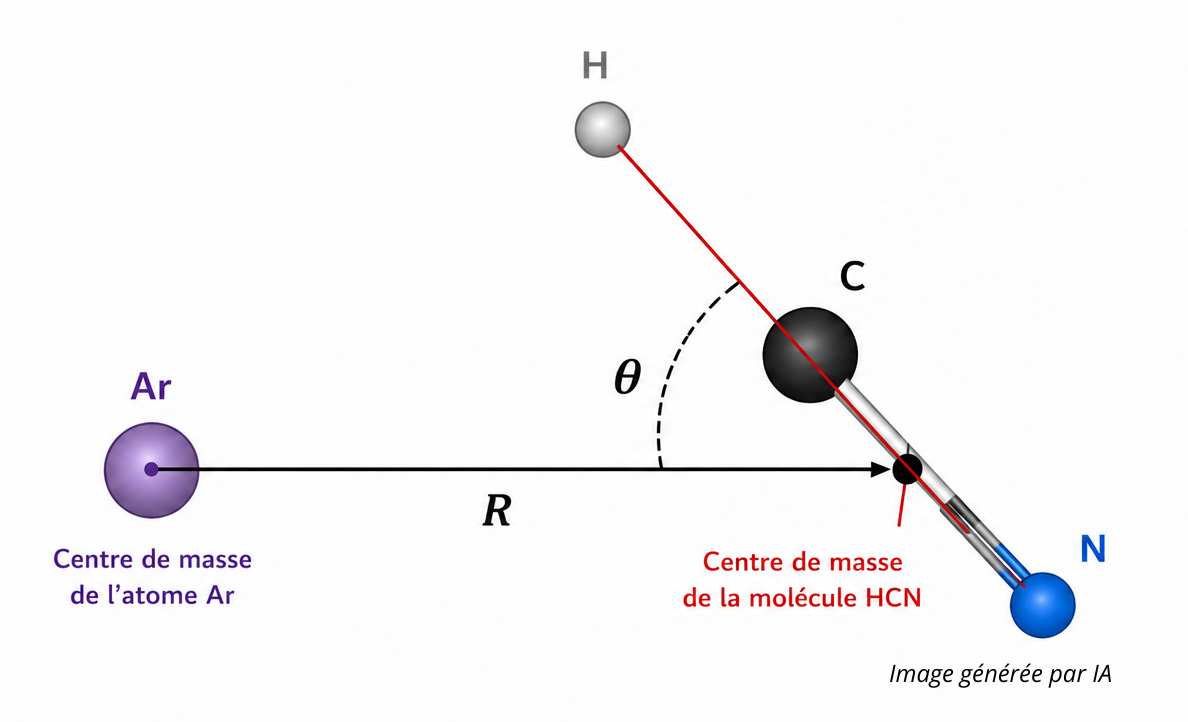
\includegraphics[width=0.55\textwidth]{../Figures/Soutenance/Systeme.png}
  \end{center}
  \caption{Illustration du complexe Ar-HCN}\label{fig:complexe}
\end{figure}

\newpage

\noindent Pour le système d'intérêt ici (voir Figure~\ref{fig:complexe} ),
on suppose que la surface de potentiel ne dépend que de $R$ et 
$\theta$ car la molécule est rigide (elle ne vibre pas) et est invariante sous
rotation autour de son axe où :\footnote{Pour le système étudié ici, le PES 
correspond à l'état fondamental électronique du complexe Ar-HCN, c'est-à-dire
l'état présentant l'énergie électronique la plus faible.}

 \begin{itemize}
   \item $R$ : Distance entre les centres de masse de A et B ;
   \item $\theta$ : Angle entre l'axe de la molécule B et le vecteur $\vec{R}$.
 \end{itemize}

\qquad

\noindent En pratique, en fixant une variable (par exemple $\theta=90$°) on
réalise des coupes de la surface d'énergie potentielle. On fixe à zéro 
l'énergie du complexe correspondant à la limite des très grandes distances ($R\to\infty$). Le signe de l'énergie
indique la nature de l'interaction entre A et B ($V > 0$ : Répulsive ; $V < 0$ : Attractive).

\begin{itemize}
  \item À courte distance $V(R,\theta)$ est très grand en raison du potentiel centrifuge (mur répulsif). 
  \item À grande distance $V(R,\theta) \to 0$ par valeurs négatives (région asymptotique).
  \item La configuration stable du système se trouve dans le puits de potentiel.
\end{itemize}

\begin{figure}[H]
  \caption{Coupe de la PES à $\theta=90$° -- Complexe Ar-HCN}\label{fig:coupe-description}
  \begin{center}
    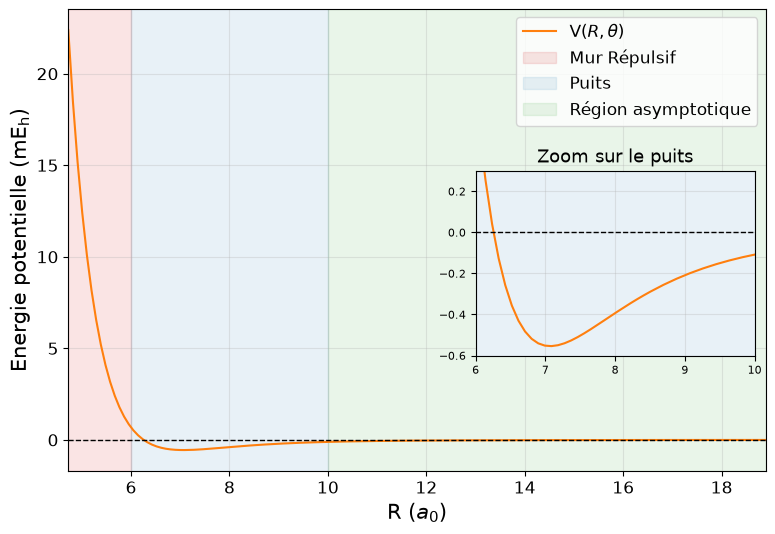
\includegraphics[width=0.60\textwidth]{../Figures/Rapport/Description-PES.png}
  \end{center}
\end{figure}


\noindent Dans ce travail, nous utilisons le milli-Hartree\footnote{1 Hartree 
= $4.36\times10^{-18}$ joules} (mE$_{h}$) comme unité d'énergie, le bohr ($a_0$) comme 
unité de distance et le degré comme unité angulaire. On précise que lorsque
$\theta=0$°, on a Ar-HCN linéaire.

\section{Sujet du stage}

\noindent La problématique de ce stage trouve son origine dans l'article de
référence publié en 2000 par R.R. Toczyłowski, F. Doloresco et S.M. Cybulski : 
\textit{Theoretical study of the He–HCN, Ne–HCN, Ar–HCN, and Kr–HCN complexes} 
\cite{ref1}.\\ 

\noindent Cet article présente des données \textit{ab initio} pour ces quatre systèmes, ainsi qu'un 
modèle analytique permettant de calculer la surface d'énergie potentielle 
$V(R,\theta)$. Ce modèle repose sur 40 paramètres qui doivent être ajustés en
fonction du système étudié. Toutefois, les auteurs ne mentionnent pas les 
valeurs numériques de ces paramètres.\\ 

\noindent Quatre ans plus tard, la thèse de doctorat de R.R. Toczyłowski (2004)
propose un jeu de paramètres pour chacun des systèmes étudiés. Cependant, une 
incohérence majeure est apparue : l'utilisation des paramètres fournis pour 
l'Argon sur le modèle analytique ne permet pas de reproduire correctement la PES
et conduit à des calculs d'états liés insatisfaisants, qui ne correspondent pas
aux résultats présentés dans l'article initial.\\

\begin{figure}[H]
    \centering
    \caption{\centering Coupes de surface pour $R$ fixé -- Comparaison des paramètres de R.R. Toczyłowski aux données \textit{ab initio}}
    \begin{subfigure}{0.45\textwidth}
        \centering
        \caption{$R=7.5$ a$_0$}
        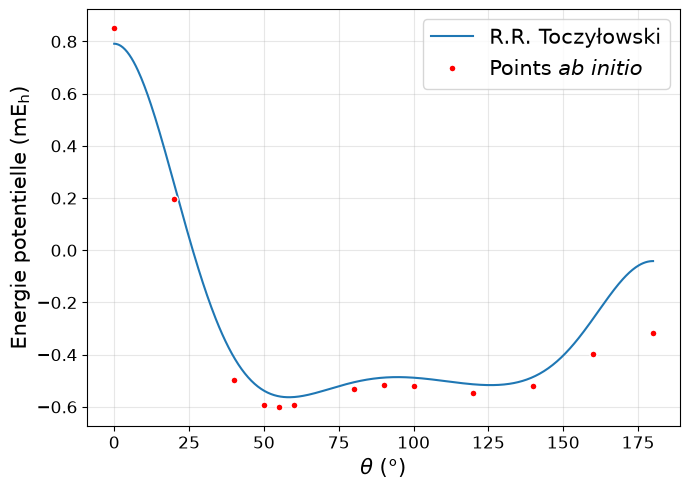
\includegraphics[width=\linewidth]{../Figures/Rapport/diff-data_Toczylowski-R7_5.png}
    \end{subfigure}
    \begin{subfigure}{0.45\textwidth}
        \centering
        \caption{$R=8.0$ a$_0$}
        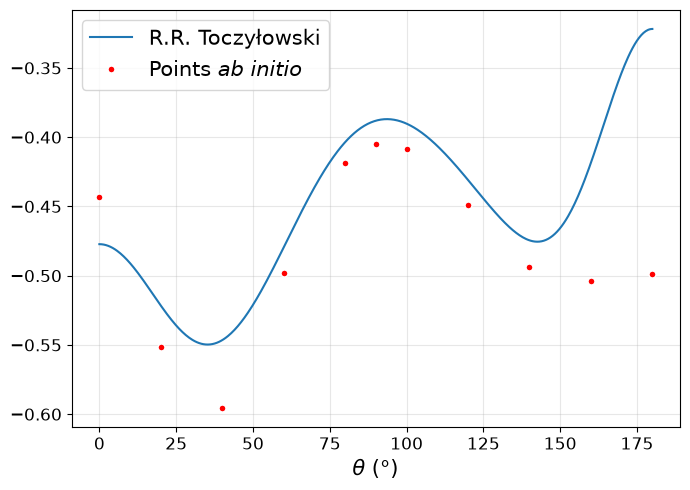
\includegraphics[width=\linewidth]{../Figures/Rapport/diff-data_Toczylowski-R8.png}
    \end{subfigure}
\end{figure}

\noindent L'objectif de ce travail est d'une part de réaliser de nouveaux ajustements de 
la surface (fits) d'énergie potentielle afin de déterminer des jeux de 
paramètres qui conduisent aux valeurs du potentiel \textit{ab initio} et
permettant de reproduire les énergies d'états liés du système, et d'autre part,
de définir des critères pertinents pour évaluer et quantifier la qualité de ces
ajustements.\\

\newpage{}
\section{Le modèle physique et ses paramètres\label{sec:modele}}

\noindent Le modèle décrivant $V(R,\theta)$ s'exprime comme la somme d'un 
terme qui décrit les interactions à courte (\textit{short}) portée ($V_{sh}$) et d'un terme 
à très longue portée ($V_{as}$) dans la région asymptotique. Entre les deux se 
trouve la région du puits où l’atome et la molécule peuvent se trouver piégés
temporairement et interagir de manière significative durant une collision.\\
$$\boxed{V(R,\theta)=V_{\mathrm{sh}}(R,\theta) + V_{\mathrm{as}}(R,\theta)}$$

où $$V_{\mathrm{sh}}=G(R,\theta)e^{D(\theta)+B(\theta)R}$$

avec $$G(R,\theta) = \sum_{l=0}^{5} (g_{0,l}+g_{1,l}R+g_{2,l}R^2+g_{3,l}R^3)P_l(\cos\theta)$$

$$D(\theta)=\sum\limits_{l=0}^{5}d_lP_l(\cos\theta) \qquad B(\theta)=\sum\limits_{l=0}^{5}b_lP_l(\cos\theta)$$\\


\noindent Les polynômes de Legendre $P_l(\cos\theta)$ forment une base des fonctions en $\theta$ et $l$
correspond au moment angulaire (entier, positif ou nul).\\ 

\noindent À très grande distance, on écrit :

$$V_{as}=f_6(\vert B(\theta)R\vert)\frac{c_0P_0(\cos\theta)+c_2P_2(\cos\theta)}{R^6}
  +f_7(\vert B(\theta)R\vert)\frac{c_1P_1(\cos\theta)+c_3P_3(\cos\theta)}{R^7}$$

\noindent La fonction d'amortissement $f_{n}(x)$ vient corriger le comportement non 
physique à courte distance du développement en $1/R^{n}$.
$$f_n(x)=1-e^{-x}\sum_{k=0}^{n}\frac{x^k}{k!}$$

\noindent Les quarante paramètres à ajuster selon le système étudié sont :
\begin{itemize}
  \item $b_{l},\;d_{l},\;g_{i,l}$ ($l=0,\dots,5$ et $i=0,1,2,3$).
  \item $c_{0},\; c_{1},\; c_{2},\; c_{3}$.
\end{itemize}

\newpage{}

\chapter{Méthodes}

\section{Les surfaces étudiées}

\begin{itemize}
  \item\label{itm:surf1} \textbf{Surface n°1 -- Ar-HCN :} Cette première surface publiée dans
    l'article de référence \cite{ref1} contient 140 points \textit{ab initio}
    sur une grille de R et $\theta$ incomplette 
    (Table~\ref{tab:Ar-HCN-Toczylowski}).
    $R$ (resp. $\theta$) prend ses valeurs entre $5$ et $15$ $a_0$ 
    (resp. $0$° et $180$°) avec un pas irrégulier.
  \item\label{itm:surf2} \textbf{Surface n°2 -- Ar-HCN :} Publiée dans le \textit{Chinese 
    Journal of Chemical Physics} \cite{ref2}, elle contient 1767 points
    \textit{ab initio} pour une grille régulière de 93 valeurs de $R$ (de 
    $3.78$ à $47.24$ $a_0$) et 19 valeurs de $\theta$ (de $0$° à $180$°).
  \item\label{itm:surf3} \textbf{Surface n°3 -- Ar-HNC : } Cette troisième surface \cite{refHNC} 
    contient une combinaison de 25000 points \textit{ab initio} et issus d'un
    premier fit sur une grille régulière de 500 valeurs de $R$ (entre $4$ et
    $30$ $a_0$) et 50 valeurs de $\theta$ (entre $0$° et $180$°).
\end{itemize}

\section{Les méthodes d'optimisation\label{sec:methodes}}

\noindent Pour effectuer nos ajustements de surface, on utilisera le langage 
Python et les fonctions du module \verb|scipy.optimize| : 
\verb|curve_fit| \cite{curve_fit}, \verb|least_squares| \cite{least_squares},
\verb|differential_evolution| \cite{differential_evolution} :\\

\begin{itemize}
  \item \texttt{curve\_fit} : Cette méthode est la plus directe pour ajuster une fonction modèle $y=f(x,p)$
  ($x=(R,\theta)$ dans notre cas). Elle repose sur des algorithmes des moindres 
  carrés non linéaires comme Levenberg-Marquardt ou Trust Region Reflective.
  
  \noindent En pratique, il suffit d'y entrer en argument notre fonction modèle, les données
  de référence ainsi que des paramètres initiaux $p_0$. La fonction convergera vers les paramètres
  optimaux les plus proches de $p_0$. Pour améliorer les résultats, on utilisera
  les options permettant de pondérer ou non le fit et faisant varier la méthode
  de minimisation utilisée par la fonction.
  
  \qquad

  \item \texttt{least\_squares} : Plus génerale que \verb|curve_fit|, cette 
    méthode travaille sur une fonction résidus fournie par l'utilisateur 
    ($\text{Res}(p)=y_{\mathrm{ref}}-y_{\mathrm{pred}}(p)$ par exemple). Elle 
    offre un niveau de contrôle plus poussé avec notamment la possibilité de 
    fixer des bornes sur les paramètres à calculer ou faire varier les fonctions
    de perte utilisées. La fonction convergera, à l'instar de \verb|curve_fit|, 
    vers le minimum local le plus proche de $p_0$.

  \qquad

  \item \texttt{differential\_evolution} : Contrairement aux deux méthodes 
    précédentes qui sont des optimisateurs locaux dépendants d'un bon choix du 
    point initial $p_0$, \verb|differential_evolution| est un algorithme 
    d'optimisation globale stochastique. Il permet d'explorer un vaste espace
    de valeurs à l'aide d'une population de solutions $p$ candidates, d'isoler
    la région du minimum global pour ensuite effectuer un affinage local.

    \noindent Comme \verb|least_squares|, elle ne prend pas directement le 
    modèle en argument mais une fonction de coût que l'on choisit.
\end{itemize}

\section{L'implémentation du modèle analytique}

\noindent Dans un premier temps, l'objectif est de développer une fonction Python fidèle 
au modèle de $V$ (Voir Section~\ref{sec:modele}).
Il est bon de préciser que dans notre programme pour la partie à courte portée, 
on prendra $e^{D(\theta)-B(\theta)R}$ au lieu de $e^{D(\theta)+B(\theta)R}$ 
car c'est ce que l'on retrouve plus communément dans la littérature\footnote{On
s'assurera d'ajuster les signes des $c_l$ lorsque nécessaire}.\\ 

\noindent Après avoir vérifié la validité des résultats fournis par la fonction,
il est essentiel d'en optimiser les performances d'exécution. En effet, les algorithmes
d'optimisation évaluant le potentiel plusieurs milliers de fois, de légères réductions 
du temps de calcul auront un impact majeur sur la durée globale du fit. Pour y parvenir,
plusieurs axes d'amélioration ont été examinés :\\

\begin{itemize}
  \item \textbf{Vectorisation NumPy :} Remplacement des boucles Python et du module 
    \verb|math| par des opérations vectorielles, permettant d'évaluer 
    simultanément l'ensemble des points $(R, \theta)$.
  \item \textbf{Optimisations algébriques :} Utilisation du schéma de Horner
    pour les polynômes $G(R, \theta)$ et $f_n$, pré-calcul explicite des factorielles, 
    et évaluation des polynômes de Legendre avec \verb|np.polynomial.legendre.legval|.
  \item \textbf{Stabilité numérique :} Utilisation de \verb|np.clip| et traitement 
    des \verb|NaN| ou infinis (\verb|np.nan_to_num|), pour prévenir
    les problèmes d'overflow lorsque les paramètres testés par les algorithmes 
    d'optimisation sont absurdes.
\end{itemize}

\noindent (Les deux versions l'implémentation sont présentées en annexe : ~\ref{lst:V_classique} -- \ref{lst:V_opt}.)

\subsection{Validation des améliorations}

\noindent Pour s'assurer de la pertinence des modifications effectués on 
applique une série de tests.\\ 

\noindent Dans un premier temps, il s'agit de vérifier que les deux
fonctions sont numériquement équivalentes. Pour ce faire, on tire aléatoirement
500 valeurs de $R$ (resp. $\theta$) entre $2$ et $10\;a_0$ (resp. $0$° et $180$°) 
selon une loi uniforme \footnote{ \texttt{numpy.random.uniform(2,10,500)}} et 
notre jeu de 40 paramètres selon une loi normale centrée réduite 
$\mathcal{N}(0,1)$ \footnote{\texttt{numpy.random.randn(40)}}. On compare 
ensuite la différence des résultats obtenus avec les deux fonctions
et on s'assure qu'elle soit suffisamment faible.

\begin{table}[H]
  \caption{Comparaison des sorties de $V_{init}$ et $V_{opt}$ ($\vert V_{init}-V_{opt} \vert$)}
  \begin{center}
    \begin{tabular}[c]{ccc}
      \hline
      \multicolumn{1}{c}{\textbf{Différence maximale}} & 
      \multicolumn{1}{c}{\textbf{Différence moyenne}} & 
      \multicolumn{1}{c}{\textbf{Écart-type de la différence}} \\
      \hline
      $1.788 \times 10^{-6}$ & $1.220 \times 10^{-8}$ & $1.090 \times 10^{-7}$\\
      \hline
    \end{tabular}
  \end{center}
\end{table}

\newpage
\noindent Dans un second temps, on évalue les gains en performance par trois
tests :
\begin{itemize}
  \item \textbf{Sur la fonction isolée :} Mesure du temps moyen d'exécution de
    $V$ sur 10000 itérations avec \verb|perf_counter|.
  \item \textbf{Sur les fonctions résidus :} Mesure du temps minimal sur 
    5 cycles de 10000 évaluations avec \verb|timeit.repeat()|(pour filtrer de
    possibles interférences de processus indépendants qui tourneraient en 
    arrière plan).
  \item \textbf{Sur la résolution complète} (\verb|least_squares|) \textbf{:} 
    Mesure du temps moyen de fit sur 1000 $p_0$ tirés aléatoirement, pour évaluer 
    le gain en conditions réelles.
\end{itemize}

\noindent Pour éviter les biais de mesure, on réalise les tests dans 
des conditions expérimentales identiques par l'intégration de \textit{warm-up}
\footnote{Exécution préliminaire que l'on ne comptabilise pas. Elle permet 
de précharger la fonction et les données dans le cache du CPU}
et le nettoyage de la mémoire.

\begin{table}[H]
  \caption{Temps d'exécution moyen par appel en secondes}
  \begin{center}
    \begin{tabular}[c]{|lcc|r|}
      \hline
      \multicolumn{1}{|c}{\textbf{}} & 
      \multicolumn{1}{c}{$V_{init}$} & 
      \multicolumn{1}{c|}{$V_{opt}$} & 
      \multicolumn{1}{c|}{Gain} \\
      \hline
      Isolée & $3.044 \times 10^{-3}$ & $8.334 \times 10^{-4}$ & $\times 3.65$ \\
      Résidus & $2.495 \times 10^{-4}$ & $1.117 \times 10^{-4}$ &  $\times 2.23$\\
      \texttt{least\_squares} & $11.336$ & $4.942$ & $\times 2.29$ \\
      
      \hline
    \end{tabular}
  \end{center}
\end{table}


\section{Les critères d'évaluation des ajustements}

\noindent Après avoir déterminé des paramètres optimaux à l'aide des différentes
méthodes, il est essentiel d'évaluer la qualité de ces ajustements. Pour s'assurer 
que le modèle incluant les nouveaux paramètres reproduise bien les données, on
effectue une première analyse graphique que l'on précisera à l'aide de métriques 
quantitatives.\\

\noindent La vérification graphique est la première étape qui permet d'écarter
les résultats aberrants et d'identifier de possibles faiblesses dans les méthodes
utilisées :
\begin{itemize}
  \item \textbf{Superposition aux données} : Comparaison directe des courbes
    obtenues aux données \textit{ab initio} à l'aide de coupes de la surface sur 
    plusieurs $R$ ou $\theta$ fixés
  \item \textbf{Cartes d'erreurs} : Représentation graphique des erreurs en 
    fonction de la géométrie
  \end{itemize}

\qquad

\noindent Ensuite, pour mesurer de manière plus précise la qualité, on introduit 
trois métriques : R², RMSE et MAE. On note $V$ les données de référence, $\bar{V}$ la moyenne de ces données et 
$\hat{V}$ les valeurs obtenues avec le modèle analytique :

\begin{itemize}
  \item \textbf{Coefficient de détermination (R²) :} Indicateur sans dimension 
    qui informe sur la qualité globale du fit. On vise à obtenir $R^2=1$.
    $$R^2 = 1 - \frac{ \sum\limits_{i=1}^{N} (V_i - \hat{V}_i)^2 }{ \sum\limits_{i=1}^{N} (V_i - \bar{V})^2 }$$
  \item \textbf{Erreur quadratique moyenne (RMSE) :} Pénalise
    les grands écarts locaux. Elle prend la même unité que les données que
    l'on cherche à évaluer.
    $$\text{RMSE} = \sqrt{ \frac{1}{N} \sum_{i=1}^{N} \left( V_i - \hat{V}_i \right)^2 }$$
  \item \textbf{Erreur absolue moyenne (MAE)} : Accorde un poids linéaire à toutes 
    les erreurs. Elle prend la même unité que les données étudiées.
    $$\text{MAE} = \frac{1}{N} \sum_{i=1}^{N} \left\vert{} V_i - \hat{V}_i \right\vert{}$$
\end{itemize}

\section{Approche alternative : Réseaux de neurones}

\noindent Durant la dernière semaine du stage, nous avons tenté d'apporter une
alternative à l'ajustement du modèle analytique. On pose un modèle semi analytique : 
$$V(R, \theta) = \sum\limits_{l=0}^{L_{\max}} c_l(R) \cdot P_l(\cos\theta)$$

\noindent On cherche à implémenter avec le module PyTorch un réseau de neurones qui 
apprendra les fonctions représentant les coefficients $c_{l}(R)$. Pour ce
faire, par souci de temps, j'ai d'abord présenté le problème à Gemini pour obtenir 
un premier prototype à ajuster si nécessaire. L'architecture de la procédure est
composée de trois étapes :
\begin{itemize}
  \item \textbf{Réseau dense :} Un réseau de neurones prend la distance $R$ 
    (que l'on normalise) en entrée et prédit le vecteur des $L_{\max} + 1$ 
    coefficients $c_l(R)$. On prend comme fonction d'activation : GELU (Gaussian
    Error Linear Unit).
  \item \textbf{Polynomes de Legendre :} Les $P_l(\cos \theta)$ sont évalués
    en parallèle.
  \item \textbf{Fusion :} L'énergie totale est le produit scalaire entre le vecteur des coefficients
    $c_l(R)$ et le vecteur des polynomes $P_l(\cos \theta)$.
\end{itemize}

\qquad

\noindent On fixe $L_{max}=18$ et on effectue l'entraînement sur la surface n°3
(\ref{itm:surf3}). Pour identifier la 
configuration optimale, on fait varier cinq hyperparamètres :

\begin{itemize}
  \item \verb|batch_size| : taille du lot.
  \item \verb|hidden_layers| : nombre et dimensions des couches cachées.
  \item \verb|learning_rate| : taux d'apprentissage.
  \item \verb|loss| : fonction que l'on cherche à minimiser (MAE ou Erreur 
    relative \ref{lst:loss_NN}).
\end{itemize}

\noindent On fixe le nombre d'époques d'entraînement à 1000 ou 2000 et on selectionne le
meilleur checkpoint.
% ------------------------------------------------------------------------------
% CHAPITRE 3 : TRAVAUX RÉALISÉS ET RÉSULTATS
% ------------------------------------------------------------------------------
\chapter{Résultats}

\section{Ajustement de la surface n°1}

\noindent Pour l'ajustement de cette première surface d'énergie potentielle \cite{ref1}, seules
\texttt{curve\_fit} et \texttt{least\_squares} ont été employées. On se satisfait d'une fonction de 
résidus standard (définie par $|V_{\text{ref}} - V_{\text{pred}}|$) pour la 
résolution via \texttt{least\_squares}. \\ 

\noindent Le processus d'ajustement n'a présenté aucune difficulté particulière.
Les résultats se sont avérés relativement stables face aux variations des 
hyperparamètres des méthodes : les modèles obtenus avec les nouveaux paramètres
sont très similaires sur le plan graphique et quantitatif 
(voir Tableau~\ref{tab:scores_toczylowski}).\\

\noindent On choisit de retenir pour cette surface le jeu de paramètres obtenu avec 
\texttt{least\_squares}, configuré avec la mise à l'échelle 
\texttt{x\_scale='jac'}\footnote{Met à l'échelle les paramètres en
utilisant le Jacobien de la fonction résidu.} et la fonction de perte 
\texttt{loss='huber'}\footnote{Réduit l'influence des valeurs 
abberrantes lors de l'optimisation.}. \\

\begin{figure}[H]
    \centering
    \caption{\centering Coupes de surface pour $R$ fixé -- Comparaison des paramètres aux données \textit{ab initio}}
    \begin{subfigure}{0.45\textwidth}
        \centering
        \caption{$R=7.5$ a$_0$}
        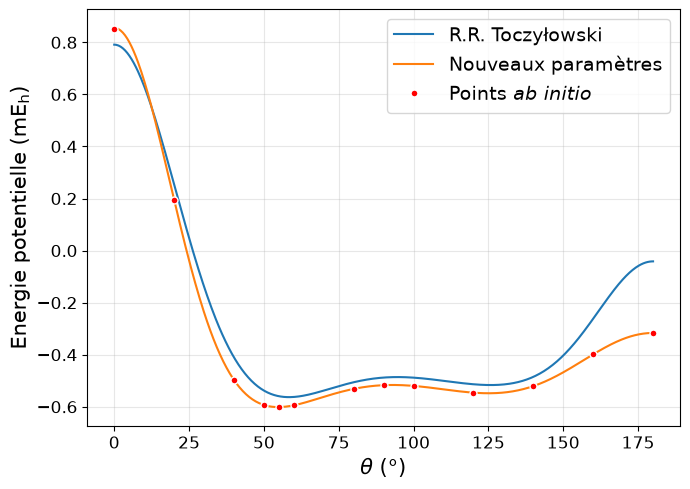
\includegraphics[width=\linewidth]{../Figures/Rapport/surf1-R7_5.png}
    \end{subfigure}
    \begin{subfigure}{0.45\textwidth}
        \centering
        \caption{$R=8.0$ a$_0$}
        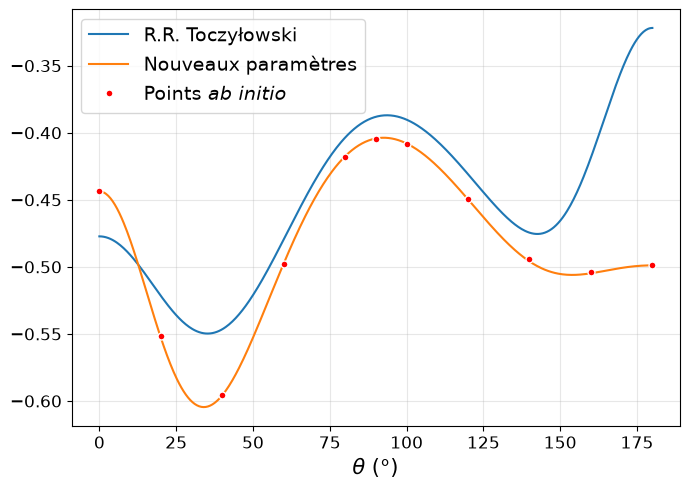
\includegraphics[width=\linewidth]{../Figures/Rapport/surf1-R8.png}
    \end{subfigure}
    \begin{subfigure}{0.45\textwidth}
        \centering
        \caption{$R=15.0$ a$_0$}
        \label{fig:coupe_R15_surf1}
        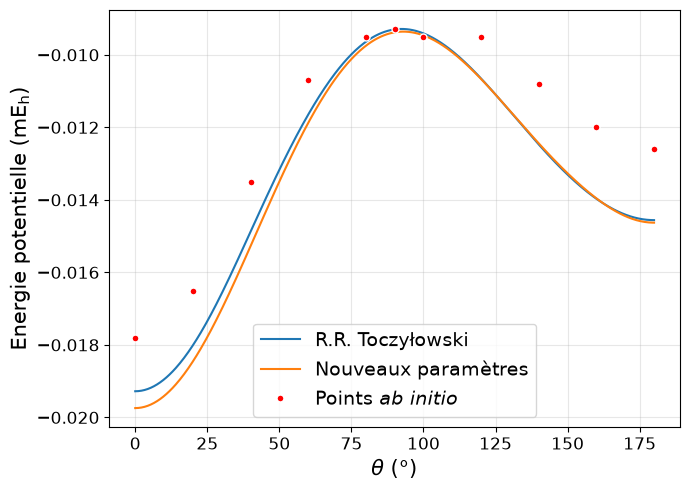
\includegraphics[width=\linewidth]{../Figures/Rapport/surf1-R15.png}
    \end{subfigure}
\end{figure}

\noindent Le gain en qualité des nouveaux paramètres sur ceux donnés par 
R.R. Toczyłowski \cite{these} ne fait pas de doute. Toutefois, en examinant
certaines coupes à grande distance (voir Figure~\ref{fig:coupe_R15_surf1}), on observe une 
difficulté du modèle à garder une erreur relative constante. En effet,
dans la région asymptotique, l'énergie d'interaction tend vers zéro. De ce fait,
un écart minime est beaucoup plus marqué.\\

\begin{figure}[H]
    \centering
    \caption{\centering Erreur relative en \% pour $\theta$ fixé}
    \begin{subfigure}{0.45\textwidth}
        \centering
        \caption{$\theta=0$°}
        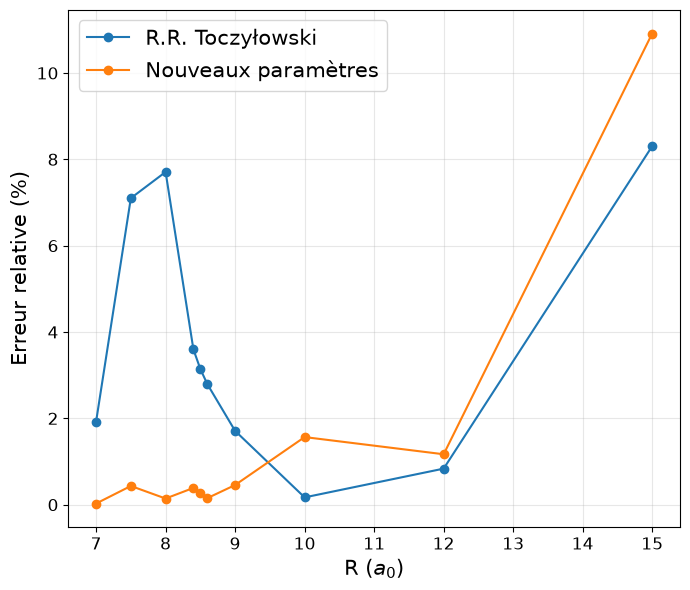
\includegraphics[width=\linewidth]{../Figures/Rapport/err-rel-surf1-T0.png}
    \end{subfigure}
    \begin{subfigure}{0.45\textwidth}
        \centering
        \caption{$\theta=90$°}
        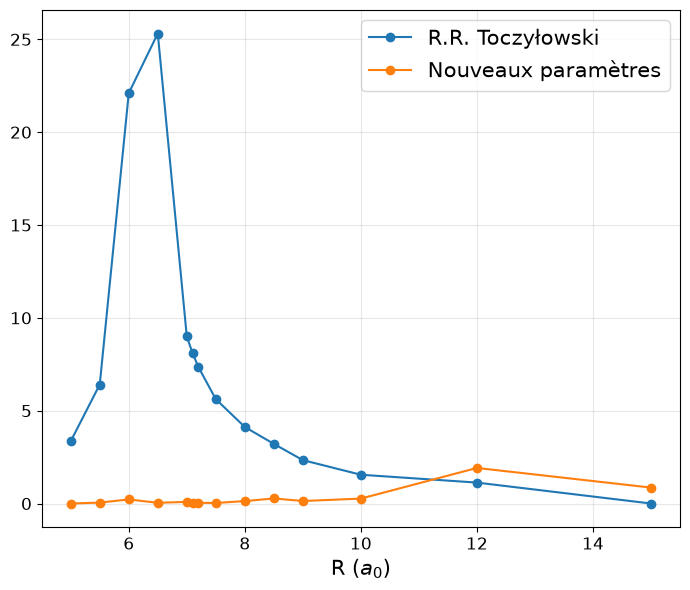
\includegraphics[width=\linewidth]{../Figures/Rapport/err-rel-surf1-T90.png}
    \end{subfigure}
    \begin{subfigure}{0.45\textwidth}
        \centering
        \caption{$\theta=180$°}
        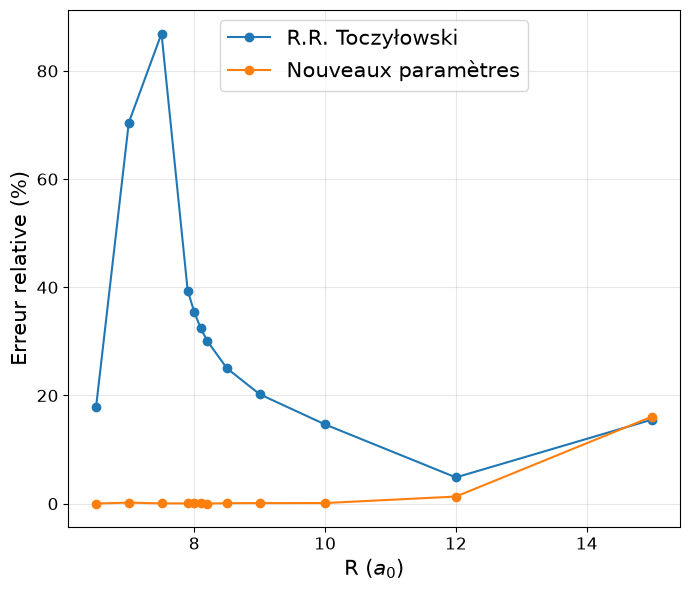
\includegraphics[width=\linewidth]{../Figures/Rapport/err-rel-surf1-T180.png}
    \end{subfigure}
\end{figure}

\noindent Des figures complémentaires appuyant les observations sont présentés
dans l'Annexe (\ref{fig:PES_surf1}).

\newpage{}
\section{Ajustement de la surface n°2}

\noindent L'ajustement de cette deuxième surface s'est avéré plus complexe 
que le précédent. Ceci est dû à un volume de données plus important et
à un intervalle d'étude plus large pour la distance R \footnote{Ce qui implique
que l'énergie potentielle prend à la fois des valeurs tres grandes et des 
valeurs qui tendent vers zéro}. On utilise les méthodes \texttt{curve\_fit, 
least\_squares et differential\_evolution}.\\

\noindent Afin d'optimiser le fit, plusieurs formulations de l'erreur ont été testées.
L'objectif de cela est de donner plus de poids aux valeurs d’énergie dans les zones 
physiquement importantes du puits et à grande distance, plus faibles que celles
de la barrière centrifuge où la fonction d’onde ne pénètre pas. On prend 
également la décision de réduire l'ensemble d'étude à des valeurs de 
$R\in[4.7,18.9]\;a_0$ :

\begin{itemize}
  \item Pour \texttt{least\_squares} : On effectue les calculs sur trois 
    fonctions résidus : l'erreur absolue et deux variantes de l'erreur relative 
  \item Pour \texttt{differential\_evolution} : On effectue les calculs sur cinq 
    fonctions de coûts : l'erreur absolue simple et des variantes pondérées
\end{itemize}

\noindent Lors de l'ajustement de cette surface, les résultats obtenus présentaient 
beaucoup plus de variations d'une configuration à l'autre.

\subsection{Le temps de calculs}

\noindent Les différentes méthodes ne sont pas égales dans le temps nécessaire
avant convergence.

\begin{table}[H]
  \caption{Temps moyen d'execution des fonctions avant convergence sur la surface n°2}\label{tab:}
  \begin{center}
    \begin{tabular}[c]{lr}
      \hline
      \multicolumn{1}{c}{Méthode} & 
      \multicolumn{1}{c}{Temps moyen en secondes} \\
      \hline
      \texttt{curve\_fit} & 2.91 \\
      \texttt{least\_squares} & 17.72\\
      \texttt{differential\_evolution} & 2600.98 \\
      \hline
    \end{tabular}
  \end{center}
\end{table}

\noindent \texttt{differential\_evolution} se distingue par son temps 
d'execution considérable.

\subsection{Analyse graphique et quantitative\label{sec:fit-surf2}}

\noindent On effectue une première sélection graphique des paramètres obtenus 
par les différentes configurations. Par exemple, il apparaît immédiatement
que la fonction \texttt{least\_squares} accompagnée d'un résidu simple (erreur
absolue) ne suffit pas (Voir Figure~\ref{fig:ls_mauvais_surf2}).\\

\noindent Finalement, sur 26 essais, on en sélectionne 4 par le biais des observations 
graphiques et des métriques.

\begin{figure}[H]
    \centering
    \caption{\centering Coupes de la PES pour les quatres paramètres sélectionnés -- Surface n°2}
    \begin{subfigure}{0.45\textwidth}
        \centering
        \caption{$R=6\;a_0$}
        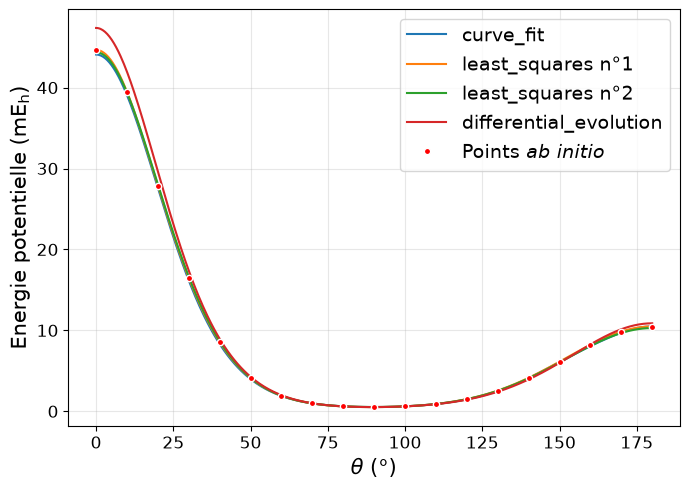
\includegraphics[width=\linewidth]{../Figures/Rapport/surf2-selec-R6.png}
    \end{subfigure}
    \begin{subfigure}{0.45\textwidth}
        \centering
        \caption{$R=8.3\;a_0$}\label{fig:surf2-selec-R8_3}
        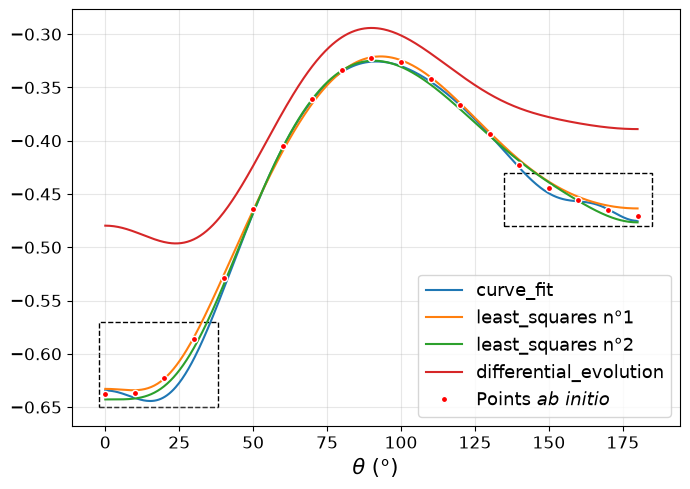
\includegraphics[width=\linewidth]{../Figures/Rapport/surf2-selec-R8_3.png}
    \end{subfigure}
    \begin{subfigure}{0.45\textwidth}
        \centering
        \caption{$R=15\;a_0$}\label{fig:surf2-selec-R15}
        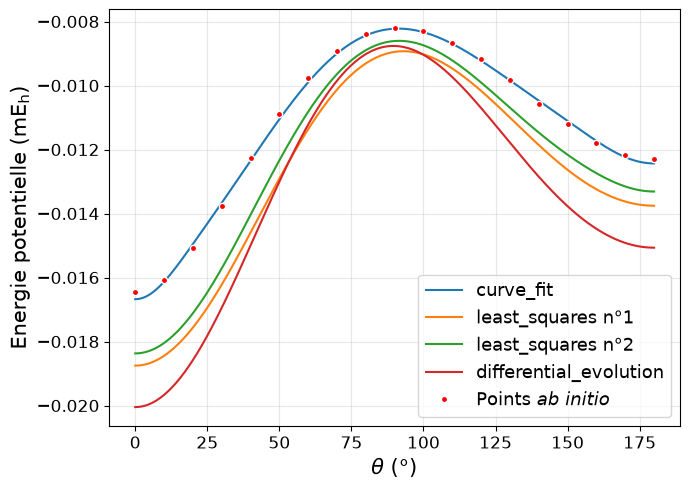
\includegraphics[width=\linewidth]{../Figures/Rapport/surf2-selec-R15.png}
    \end{subfigure}
\end{figure}

\noindent On écarte les paramètres obtenus via 
\texttt{differential\_evolution} dont les résultats sont visiblement peu
satisfaisants. Les autres paramètres donnent des résultats similaires avec
chacun ses caractéristiques.
Par exemple, les paramètres issus de \texttt{curve\_fit} sont particulièrement
bons pour $R$ grand (Figure~\ref{fig:surf2-selec-R15}). Néanmoins,
ils présentent une certaine faiblesse aux extrémités pour certaines valeurs de 
$R$ (voir Figure~\ref{fig:surf2-selec-R8_3}).\\

\noindent On se sert des métriques pour faire un choix et on introduit deux
variantes de la MAE : une version pondérée qui donne plus d'importance au 
puits de potentiel et une version réduite qui est seulement calculée sur 
l'intervalle $[-1,1]\;\text{mE}_h$.

\begin{table}[ht]
\centering
\caption{Scores relatifs aux paramètres sélectionnés pour la surface n°2}
\resizebox{\textwidth}{!}{%
\begin{tabular}{lccccc}
\toprule
\textbf{Méthode} & \textbf{R$^2$} & \textbf{RMSE (mE$_{h}$)} & \textbf{MAE (mE$_{h}$)} & \textbf{MAE pondérée} & \textbf{MAE intervalle} \\
\midrule
curve\_fit  & 0.99740565 & 2.07509219 & 0.26710798 & 0.00684283 & 0.00200393 \\
least\_squares n°1  & 0.99999794 & 0.05845209 & 0.01465815 & 0.00356479 & 0.00323640 \\
least\_squares n°2 & 0.98918260 & 4.23725241 & 0.42103226 & 0.00664192 & 0.00237813 \\
differential\_evolution & 0.98121175 & 5.58426445 & 0.87852188 & 0.03881056 & 0.02333764\\
\bottomrule
\end{tabular}
}
\end{table}

\noindent On finit par choisir les paramètres obtenus avec \texttt{curve\_fit}
(Tableau~\ref{tab:best_params_surf2})
car bien qu'ils ne se démarquent pas sur le plan quantitatif, lorsque l'on
s'intéresse aux erreurs relatives aux alentours des énergies minimales, il 
apparaît comme meilleur (voir Figure~\ref{fig:PES-surface-2}).

\section{Nouveau système : Ar-HNC}

\noindent J'effectue un dernier ajustement "classique" sur la surface n°3 
(Section~\ref{itm:surf3}).
Les difficultés rencontrées sont intrinsèquement
les mêmes que pour la surface n°2. On réitère donc la méthodologie de la 
Section~\ref{sec:fit-surf2} 
et on compare les deux surfaces. (Paramètres appliqués au modèle : Table~\ref{tab:best_params_surf3})

\begin{figure}[H]
    \centering
    \caption{\centering Coupes de la PES pour les surfaces n°2 et n°3}
    \begin{subfigure}{0.45\textwidth}
        \centering
        \caption{$\theta=0$°}
        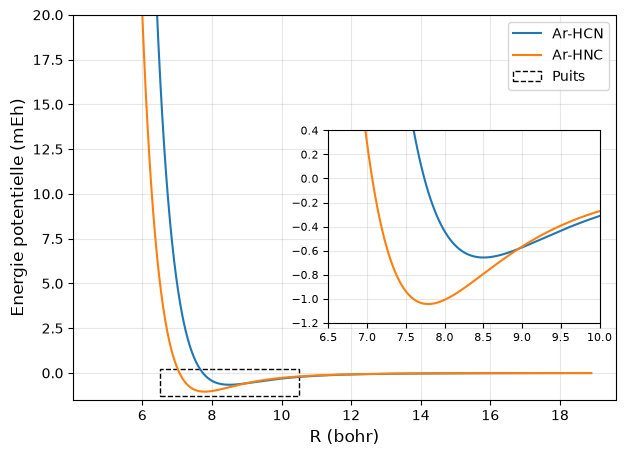
\includegraphics[width=\linewidth]{../Figures/Soutenance/HCN-HNC-T0.png}
    \end{subfigure}
    \begin{subfigure}{0.45\textwidth}
        \centering
        \caption{$\theta=90$°}
        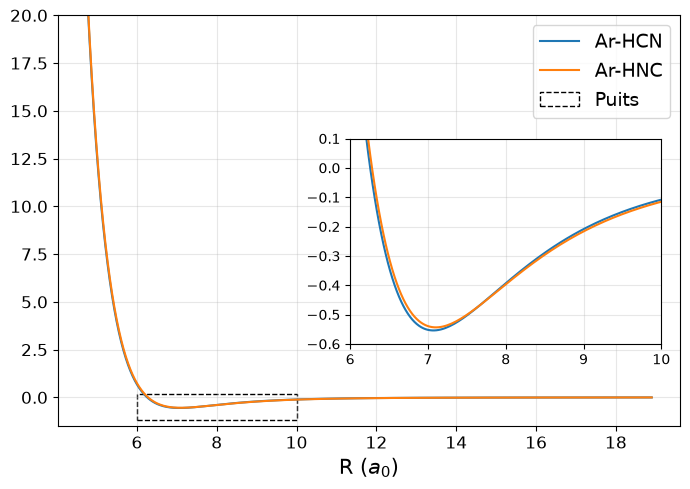
\includegraphics[width=\linewidth]{../Figures/Soutenance/HCN-HNC-T90.png}
    \end{subfigure}
    \begin{subfigure}{0.45\textwidth}
        \centering
        \caption{$\theta=180$°}
        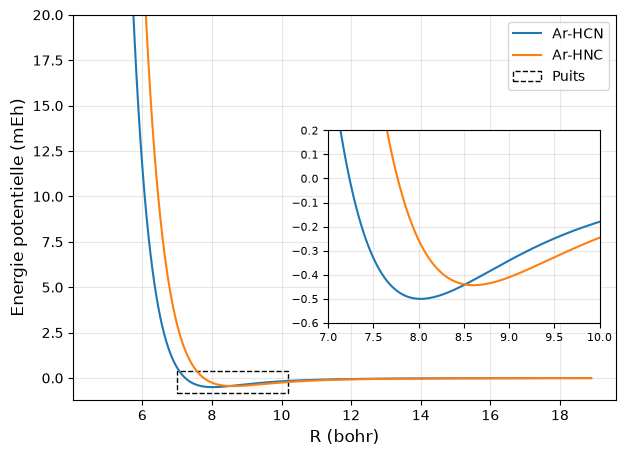
\includegraphics[width=\linewidth]{../Figures/Soutenance/HCN-HNC-T180.png}
    \end{subfigure}
\end{figure}

\noindent Ces figures mettent en évidence le comportement géométrique lié à l'inversion 
des atomes de carbone et d'azote. Lorsque l'argon s'approche par les extrémités
de la molécule (à $0^\circ$ et $180^\circ$), il fait face à une configuration
différente d'un système à l'autre. Ainsi il y a un phénomène d'inversion des
puits de potentiel qui apparaît. En revanche, à $90$° le centre de la molécule
est perçu de la même manière dans les deux cas, d'où la superposition des courbes.

\newpage{}
\section{Réseaux de neurones}

\noindent L'apprentissage du réseau s'est effectué sur la surface n°3 spécifiquement en
raison du grand volume de données qu'il contient pour pouvoir entraîner notre
modèle dans les meilleures conditions possible. Sur le plan technique, 
l'implémentation sur PyTorch a permis de profiter de l'accélération GPU
\footnote{CUDA 12. -- Nvidia GeForce GTX 750ti}. Ainsi, cette méthode a pu rester très compétitive (temps 
d'entraînement) par rapport aux algorithmes précédents.\\

\begin{figure}[H]
    \centering
    \caption{\centering Coupes de la PES pour les surfaces n°2 et n°3}
    \begin{subfigure}{0.45\textwidth}
        \centering
        \caption{$\theta=0$°}
        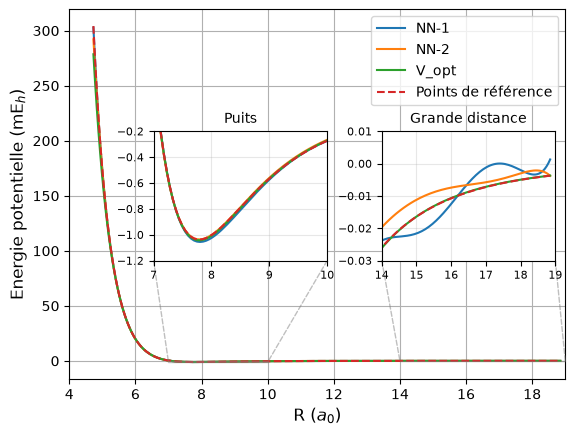
\includegraphics[width=\linewidth]{../Figures/Rapport/NN-T0.png}
    \end{subfigure}
    \begin{subfigure}{0.45\textwidth}
        \centering
        \caption{$\theta=90$°}
        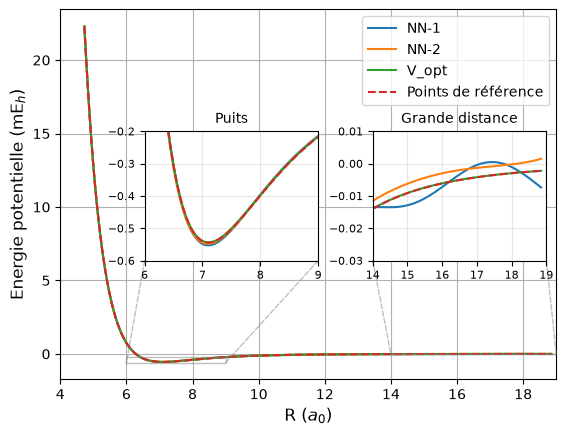
\includegraphics[width=\linewidth]{../Figures/Rapport/NN-T90.png}
    \end{subfigure}
    \begin{subfigure}{0.45\textwidth}
        \centering
        \caption{$\theta=180$°}
        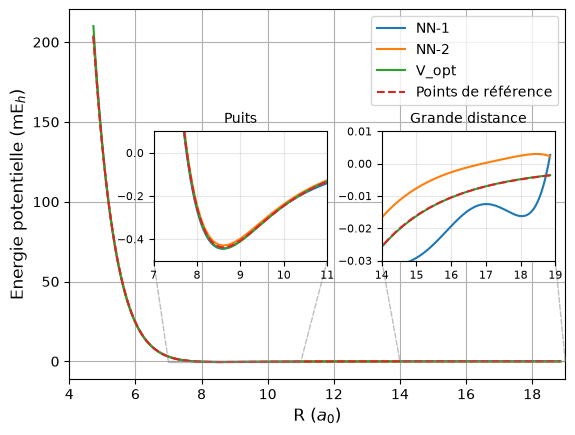
\includegraphics[width=\linewidth]{../Figures/Rapport/NN-T180.png}
    \end{subfigure}
\end{figure}

\noindent Bien que le réseau modélise correctement la région du puits, les
figures ci-dessus mettent en évidence ses limites à grande distance, à savoir,
des phénomènes d'oscillation et l'apparition de valeurs d'énergie positives.
Ceci est dû au fait que le réseau n'est pas informé de la physique du système
contrairement au modèle analytique.


\chapter{Analyse critique et perspectives}

\section{Le choix des méthodes d'optimisation}

\noindent La comparaison des trois algorithmes (\ref{sec:methodes}) a mis en
évidence le fait que \texttt{differential\_evolution} a produit les résultats
les moins satisfaisants graphiquement et quantitativement, et ce, malgré sa
capacité théorique à mieux échapper aux minima locaux en plus de présenter
des coûts de calculs largement moins intéressants que les deux autres méthodes :
2601 secondes contre 17.7 secondes pour \texttt{least\_squares}.\\

\noindent L'inefficacité de \texttt{differential\_evolution} pourrait s'expliquer en
premier lieu par une mauvaise configuration des hyperparamètres de la fonction
et/ou de l'espace de recherche des paramètres \footnote{S'assurer d'un choix de
bornes pertinent}, mais également par le fait que les surfaces étudiées étaient
probablement plus favorables à l'utilisation de méthodes locales rendant un 
choix réfléchi de paramètres initiaux \footnote{Comme les paramètres donnés par R.R. Toczyłowski
\ref{tab:params_toczylowski}}
nettement plus intéressant.

\section{La qualité des données de référence}

\noindent Le fait de faire varier la nature des données d'entrée a permis de
mettre en évidence l'influence de leurs caractéristiques sur la qualité des 
ajustements.\\ 

\noindent Par exemple, la surface n°1 (Section~\ref{itm:surf1})
étant composée d'un faible nombre de points rend fragile la fiabilité des
paramètres en dehors des zones denses. Cette fragilité reste anecdotique, du
fait que les points sont répartis de manière à viser les régions les plus 
pertinentes de la surface.\\

\noindent Pour la surface n°3 (Section~\ref{itm:surf3})
le caractère hybride du jeu de données (points \textit{ab initio} et issus d'un
précédent ajustement via un autre modèle) est potentiellement source 
d'introduction d'un biais dans l'évaluation de qualité des paramètres\footnote{
On effectue l'ajustement d'une surface déjà ajustée}. La démarche reste justifiée
en raison de l'objectif premier de l'étude de cette surface qui était simplement
de fournir des paramètres capables de fitter les données ab initio.\\ 

\noindent Enfin, les surfaces 2 et 3 incluent des distances $R$ extrêmes dont
l'intérêt physique est négligeable\footnote{Le comportement à très courte et très longue distance 
est connu et ne nécessite pas de détails}. Les différences extrêmes d'échelle de
l'énergie que cela engendre ajoutent une complexité qui peut facilement être 
évitée en réduisant l'échantillon aux distances physiquement pertinentes.

\section{Approche par les réseaux de neurones}

\noindent Cette étape confirme une limite propre aux modèles basés purement sur
les données. En effet, bien que le réseau reproduise correctement la région du
puits de potentiel, il tend à diverger rapidement à grande distance (présentant 
des puits locaux non physiques et des valeurs d'énergie positives). L'absence 
de contraintes permettant de respecter les comportements physiques du système
pénalise cette approche et valorise l'utilisation plus traditionnelle d'un 
modèle analytique.\\

\noindent Ce constat reste à nuancer car cette approche n'a peut-être pas 
eu l'occasion de pleinement faire ses preuves, et l'optimisation du réseau 
aurait pu être poussée davantage notamment via l'introduction d'autres 
fonctions de perte plus adaptées ou l'utilisation d'autres combinaisons
d'hyperparamètres. Il convient également de noter que l'exploration de ces 
configurations s'est faite sur une carte graphique relativement ancienne\footnote{Nvidia 
GeForce GTX 750ti 2Go: carte sortie en 2014 -- Particulièrment modeste au regards
des standards actuels}, ce qui a potentiellement été un facteur limitant dans 
l'ampleur de la recherche d'hyperparamètres.\\ 


\noindent D'autres pistes d'amélioration pourraient éventuellement donner une
chance à cette méthode :

\begin{itemize}
  \item \textbf{Intégration de contraintes physiques :} En pénalisant directement
    les comportements non physiques (\textit{Réseaux neuronaux informés par la physique}).
  \item \textbf{Nouvelle architecture :} En ayant recours à un réseau appliquant 
    une correction pour compenser les erreurs du modèle analytique.
  \item \textbf{Système à dimension supérieure :} Là où les réseaux de neurones
    gagneraient en pertinence et en compétitivité serait sur des problèmes
    impliquant davantage de degrés de liberté, par exemple en intégrant les 
    vibrations intramoléculaires au système d'étude.
\end{itemize}


% ------------------------------------------------------------------------------
% CHAPITRE 4 : BILAN DU STAGE:width
% ------------------------------------------------------------------------------
\chapter{Conclusion}

\section{Bilan Technique et Scientifique}

\noindent Ce stage a tout d'abord été marqué par mon implémentation du modèle analytique
permettant de modéliser les surface d'énergie potentielle pour les systèmes
composés d'un atome et d'une molécule linéaire. Cette implémentation m'a
également demandé un important travail d'optimisation pour rendre viables les
futurs ajustements de surface. Ensuite, ce programme a pu être utilisé comme base dans
la détermination de nouveaux paramètres validés par nos tests et par calculs
d'états liés, permettant de résoudre les erreurs repérées dans les
travaux de référence \cite{ref1}. J'ai également effectué un travail de 
comparaison des méthodes d'optimisation (comme \texttt{curve\_fit, 
least\_squares} et \texttt{differential\_evolution}) mettant la lumière sur
l'importance du choix des algorithmes on fonction des données d'étude. 
Enfin, le projet a été vecteur d'une première approche personnelle sur les 
réseaux de neurones, leur potentiel ainsi que leurs limites.

\section{Bilan Personnel et Professionnel}

\noindent Sur le plan technique, ce projet a été source de développement et 
d'approfondissement de mes compétences en Python pour le calcul scientifique
(avec les bibliothèques NumPy, SciPy et PyTorch) mais aussi pour la visualisation
de données complexes (notamment via Matplotlib et Plotly) afin de faciliter
l'interprétabilité des résultats. J'ai également pu solidifier mes pratiques
de développement en travaillant sur l'environnement Linux et par l'utilisation
d'outils de gestion de versions (Git). Il était nécessaire au quotidien de 
faire preuve d'organisation, de rigueur et d'autonomie pour structurer
l'évolution du code et gérer les erreurs d'implémentation rencontrées. Enfin,
la rédaction de résumés intermédiaires au cours du stage ainsi que la 
préparation de la soutenance et de ce rapport ont été une occasion de travailler
ma communication scientifique.\\

\noindent \textit{L'ensemble de mon travail est accessible sur la page GitHub :
\url{https://github.com/Amynek/Stage-M1}.}



% ------------------------------------------------------------------------------
% BIBLIOGRAPHIE
% ------------------------------------------------------------------------------
%\chapter*{Bibliographie}
\addcontentsline{toc}{chapter}{Bibliographie}

\begin{thebibliography}{99}
    \bibitem{structure} Site officiel de l'Institut de Physique de Rennes : \url{https://ipr.univ-rennes.fr/linstitut/presentation-de-lipr}
    \bibitem{ref1} Toczylowski R R, Doloresco F and Cybulski S M 2001 J. Chem. Phys. 114 851–864
    \bibitem{ref2} T. Liman, S. Tong, N. Chuangang, C. Xialin -- 2026 -- \textit{Ab initio Potential Energy Surfaces and Low-Temperature
    Collisional Dynamics for Rotational De-excitation of HNC and HCN by Ar} -- Chinese Journal of Chemical Physics, sous presse.
    \bibitem{these} R.R. Toczylowski -- 2004 -- \textit{Doctoral thesis} -- Miami University.
    \bibitem{refHNC} Robin et Lique, communication privée.
    \bibitem{curve_fit} Documentation officielle Scipy \url{https://docs.scipy.org/doc/scipy/reference/generated/scipy.optimize.curve_fit.html}.
    \bibitem{least_squares} Documentation officielle Scipy \url{https://docs.scipy.org/doc/scipy/reference/generated/scipy.optimize.least_squares.html}.
    \bibitem{differential_evolution} Documentation officielle Scipy \url{https://docs.scipy.org/doc/scipy/reference/generated/scipy.optimize.differential_evolution.html}.
\end{thebibliography}

% ------------------------------------------------------------------------------
% ANNEXES (OPTIONNEL)
% ------------------------------------------------------------------------------
\appendix
\chapter{Annexes}

\section{Tableaux}

\begin{table}[H]
  \caption{Énergies d'interaction (en $\mu E_{h}$) calculées pour Ar-HCN \cite{ref1}}\label{tab:Ar-HCN-Toczylowski}
  \begin{center}
  \resizebox{\textwidth}{!}{%
    \begin{tabular}[c]{rrrrrrrrrrrr}
      \hline\hline
      \multicolumn{1}{c}{$R[a_0]$} & 
      \multicolumn{1}{c}{$\theta=0$°} &
      \multicolumn{1}{c}{$20$°} &
      \multicolumn{1}{c}{$40$°} &
      \multicolumn{1}{c}{$60$°} &
      \multicolumn{1}{c}{$80$°} &
      \multicolumn{1}{c}{$90$°} &
      \multicolumn{1}{c}{$100$°} &
      \multicolumn{1}{c}{$120$°} &
      \multicolumn{1}{c}{$140$°} &
      \multicolumn{1}{c}{$160$°} &
      \multicolumn{1}{c}{$180$°} \\
      \hline
      $5.00$ & & & & & $13296.3$ & $12669.6$ & $13566.2$ & & & & \\
      $5.50$ & & & & $8192.8$ & $4201.3$ & $3923.2$ & $4239.0$ & $7091.8$ & & & \\
      $6.00$ & & & $9684.6$ & $2247.9$ & $780.0$ & $684.1$ & $787.6$ & $1807.4$ & $4728.6$ & $9283.5$ & \\
      $6.50$ & & $10758.0$ & $2751.7$ & $98.4$ & $-333.3$ & $-351.9$ & $-323.4$ & $-17.2$ & $987.7$ & $2639.5$ & $3561.2$ \\
      $7.00$ & $5216.5$ & $2908.0$ & $240.4$ & $-524.3$ & $-576.3$ & $-567.9$ & $-564.2$ & $-512.8$ & $-235.5$ & $293.2$ & $601.2$ \\
      $7.50$ & $851.7$ & $195.1$ & $-498.3$ & $-593.8$ & $-531.2$ & $-516.9$ & $-519.4$ & $-546.2$ & $-519.5$ & $-397.9$ & $-316.6$ \\
      $8.00$ & $-443.1$ & $-551.4$ & $-595.6$ & $-498.1$ & $-418.3$ & $-404.8$ & $-408.2$ & $-449.2$ & $-494.0$ & $-503.9$ & $-498.6$ \\
      $8.50$ & $-668.8$ & $-625.9$ & $-502.9$ & $-378.4$ & $-309.4$ & $-299.1$ & $-301.9$ & $-338.8$ & $-392.9$ & $-434.8$ & $-448.9$ \\
      $9.00$ & $-583.2$ & $-515.2$ & $-380.7$ & $-275.6$ & $-223.2$ & $-215.9$ & $-218.7$ & $-247.0$ & $-292.8$ & $-333.8$ & $-349.6$ \\
      $10.00$ & $-315.5$ & $-274.0$ & $-198.1$ & $-142.7$ & $-117.0$ & $-113.4$ & $-114.9$ & $-129.2$ & $-155.0$ & $-178.5$ & $-188.4$ \\
      $12.00$ & $-83.1$ & $-74.2$ & $-56.8$ & $-43.1$ & $-36.5$ & $-35.6$ & $-35.2$ & $-40.5$ & $-47.5$ & $-54.0$ & $-56.9$ \\
      $15.00$ & $-17.8$ & $-16.5$ & $-13.5$ & $-10.7$ & $-9.5$ & $-9.3$ & $-9.5$ & $-9.5$ & $-10.8$ & $-12.0$ & $-12.6$ \\
      \\
      \multicolumn{1}{c}{} & 
      \multicolumn{1}{c}{$0$°} &
      \multicolumn{1}{c}{$45$°} &
      \multicolumn{1}{c}{$50$°} &
      \multicolumn{1}{c}{$55$°} &
      \multicolumn{1}{c}{$60$°} &
      \multicolumn{1}{c}{$90$°} &
      \multicolumn{1}{c}{$95$°} &
      \multicolumn{1}{c}{$100$°} &
      \multicolumn{1}{c}{$105$°} &
      \multicolumn{1}{c}{$180$°} &
      \multicolumn{1}{c}{} \\        
      \hline
      $7.00$ & & & & & & & $-565.9$ & $-564.2$ & $-560.8$ & & \\
      $7.10$ & & & & & & $-569.8$ & $-568.2$ & $-567.7$ & $-567.4$ & & \\
      $7.20$ & & & & & & $-564.0$ & $-562.8$ & $-563.4$ & $-565.4$ & & \\
      $7.30$ & & & & $-584.5$ & $-599.3$ & & & & & & \\
      $7.40$ & & & $-575.3$ & $-598.0$ & $-600.5$ & & & & & & \\
      $7.50$ & & & $-593.5$ & $-600.8$ & & & & & & & \\
      $7.60$ & & $-586.4$ & $-599.6$ & $-595.7$ & & & & & & & \\
      $7.70$ & & & $-596.8$ & & & & & & & & \\
      $7.90$ & & & & & & & & & & $-490.3$ & \\
      $8.10$ & & & & & & & & & & $-498.5$ & \\
      $8.20$ & & & & & & & & & & $-492.5$ & \\
      $8.40$ & $-662.1$ & & & & & & & & & & \\
      $8.60$ & $-664.2$ & & & & & & & & & & \\ 
      \hline
      \hline
    \end{tabular}
  }
  \end{center}
\end{table}

\begin{table}[H]
  \caption{Paramètres donnés par R.R. Toczyłowski \cite{these} pour Ar-HCN}\label{tab:params_toczylowski}
  \begin{center}
    \begin{tabular}[c]{lrrrrrr}
      \hline
      \multicolumn{1}{c}{\textbf{k}} & 
      \multicolumn{1}{c}{\textbf{0}} & 
      \multicolumn{1}{c}{\textbf{1}} & 
      \multicolumn{1}{c}{\textbf{2}} & 
      \multicolumn{1}{c}{\textbf{3}} & 
      \multicolumn{1}{c}{\textbf{4}} & 
      \multicolumn{1}{c}{\textbf{5}} \\
      \hline
      $b_k$ & 1.48547 &  0.05926 & -0.07533 & 0.12892 & 0.04978 & -0.00004 \\
      $c_k$ & -134348.77 &  -281277.47 &  -57041.638 & -116961.41 \\
      $d_k$ &  14.23209 & 0.99248 & 0.88287 & 0.70551 &  0.38213 & 0.06818\\
      $g_{k,0}$ & 0.06053 & -0.12937 &  0.07849 & -0.05992 & 0.04541 & 0.03519 \\
      $g_{k,1}$ & 0.00640 & 0.04016 & -0.02325 & 0.02468 & -0.02338 & -0.01536 \\
      $g_{k,2}$ & -0.00277 & -0.00416 & 0.00221 & -0.00239 & 0.00392 & 0.00207 \\
      $g_{k,3}$ & 0.00013 & 0.00015 & -0.00006 & 0.00003 & -0.00021 & -0.00009  \\
      
      \hline
    \end{tabular}
  \end{center}
\end{table}

\begin{table}[H]
  \caption{Paramètres calculés retenus pour la surface n°1}\label{tab:best_params_1}
  \begin{center}
  \resizebox{\textwidth}{!}{%
    \begin{tabular}[c]{lrrrrrr}
      \hline
      \multicolumn{1}{c}{\textbf{k}} & 
      \multicolumn{1}{c}{\textbf{0}} & 
      \multicolumn{1}{c}{\textbf{1}} & 
      \multicolumn{1}{c}{\textbf{2}} & 
      \multicolumn{1}{c}{\textbf{3}} & 
      \multicolumn{1}{c}{\textbf{4}} & 
      \multicolumn{1}{c}{\textbf{5}} \\
      \hline
      $b_k$ & 1.4834580 & 0.1119314 & -0.0328287 & 0.0943807 & 0.0338085 & -0.0046286 \\
      $c_k$ & 135784.75 & -325678.75 & -57995.352 & -125775.77 \\
      $d_k$ &  14.271529 & 1.2096562 & 1.1275672 & 0.4664125 & 0.2638973 & 0.0436920\\
      $g_{k,0}$ & 0.0488596 & -0.1666354 & 0.0319881 & -0.0324706 & 0.0148494 & 0.0101494\\
      $g_{k,1}$ & 0.0098652 & 0.0557663 & -0.0097596 & 0.0149440 & -0.0099116 & -0.0055877 \\
      $g_{k,2}$ & -0.0032256 & -0.0059935 & 0.0012635 & -0.0013006 & 0.0020280 & 0.0008308 \\
      $g_{k,3}$ & 0.0001521 & 0.0002130 & -0.0000591 & -0.0000091 & -0.0001256 & -0.0000343  \\
      
      \hline
    \end{tabular}
  }
  \end{center}
\end{table}

\begin{table}[H]
  \caption{\centering Scores relatifs aux paramètres obtenus \\ pour chaque méthode sur la surface n°1 }\label{tab:scores_toczylowski}
  \begin{center}
  \resizebox{\textwidth}{!}{%
    \begin{tabular}[c]{lccc}
      \hline
      \multicolumn{1}{c}{\textbf{Paramètres}} & 
      \multicolumn{1}{c}{\textbf{R²}} & 
    \multicolumn{1}{c}{\textbf{RMSE} (mE$_h$)} & 
      \multicolumn{1}{c}{\textbf{MAE} (mE$_h$)} \\
      \hline
      R.R. Toczyłowski & 0.99735712 & 0.14053713 & 0.07967955 \\
      \texttt{curve\_fit + method='lm'} & 0.99999981 & 0.00119432 & 0.00087006 \\
      \texttt{curve\_fit + method='lm' + sigma=V\_ref} &  0.99999102 & 0.00819351  & 0.00276581\\
      \texttt{curve\_fit + method='trf'} & 0.99999976 & 0.00133452 & 0.00094147 \\
      \texttt{curve\_fit + method='trf' + sigma=V\_ref} & 0.99992474 & 0.02371524 & 0.00688135 \\
      \texttt{least\_squares} & 0.99999976 & 0.00133410  & 0.00094176\\
      \texttt{least\_squares + x\_scale='jac'} & 0.99999981 & 0.00119432 & 0.00087006\\
      \texttt{least\_squares + x\_scale='jac' + loss='soft\_l1'} & 0.99999981 & 0.00119432 & 0.00087005\\
      \textbf{\texttt{least\_squares + x\_scale='jac' + loss='huber'}}& \textbf{0.99999981} & \textbf{0.00119432} & \textbf{0.00087006}\\
      \hline
    \end{tabular}
  }
  \end{center}
\end{table}

\begin{table}[H]
\centering
\caption{Paramètres sélectionnés pour la surface n°2}
\label{tab:best_params_surf2}
\resizebox{\textwidth}{!}{%
\begin{tabular}{lrrrrrr}
\toprule
\textbf{k} & \textbf{0} & \textbf{1} & \textbf{2} & \textbf{3} & \textbf{4} & \textbf{5} \\
\midrule
$b_k$  &  1.4330263 &  0.0357134 & -0.1607479 & -0.0121635 & -0.0457344 &  0.0148357 \\
$c_k$  & -119043.41 & -234068.29 & -42215.107 & -124876.08 &   & \\
$d_k$  &  13.375954 & -0.3189892 & 1.4543580 & -0.2674760 & -0.0000507 & 0.0396656 \\
$g_{k,0}$ & 0.1870131 & 0.0429435 & 0.0324089 & 0.2536370 & 0.1716549 & 0.0419323 \\
$g_{k,1}$ & -0.0181239 & 0.0155891 & -0.0306494 & -0.0901479 & -0.0594787 & -0.0183153 \\
$g_{k,2}$ & -0.0009014 & -0.0039747 & 0.0040008 & 0.0100961 & 0.0069931 & 0.0024678 \\
$g_{k,3}$ & 0.0000112 & 0.0001696 & -0.0000549 & -0.0003445 & -0.0002870 & -0.0001049 \\
\bottomrule
\end{tabular}
}
\end{table}

\begin{table}[H]
\centering
\caption{Paramètres sélectionnés pour la surface n°3}
\label{tab:best_params_surf3}
\resizebox{\textwidth}{!}{%
\begin{tabular}{lrrrrrr}
\toprule
\textbf{k} & \textbf{0} & \textbf{1} & \textbf{2} & \textbf{3} & \textbf{4} & \textbf{5} \\
\midrule
$b_k$  &  1.3927515 & 0.0969300 & -0.0598408 & 0.0979666 & 0.0440331 & -0.0066774 \\
$c_k$  & -135783.59 & -325692.43 & -57995.311 & -125784.85 \\
$d_k$  &  14.356223 & 1.2155114 & 1.1171694 & 0.4725050 & 0.2654722 & 0.0397397 \\
$g_{k,0}$ & 0.0421958 & -0.0743663 & 0.0044449 & -0.0055691 & 0.0510967 & -0.0110268 \\
$g_{k,1}$ & 0.0012035 & 0.0230020 & 0.0016336 & -0.0014390 & -0.0208052 & 0.0056295 \\
$g_{k,2}$ & -0.0014415 & -0.0031206 & -0.0005978 & 0.0011483 & 0.0027666 & -0.0009803 \\
$g_{k,3}$ & 0.0000770 & 0.0001784 & 0.0000445 & -0.0001172 & -0.0001208 & 0.0000578 \\
\bottomrule
\end{tabular}
}
\end{table}


\clearpage{}
\newpage{}
\section{Figures}
\begin{figure}[H]
    \centering
    \caption{\centering Contour plot de l'énergie potentielle pour Ar-HCN (surface n°1)}
    \label{fig:PES_surf1}
    \begin{subfigure}{0.49\textwidth}
        \centering
        \caption{Paramètres de R.R. Toczyłowski (\ref{tab:params_toczylowski})}
        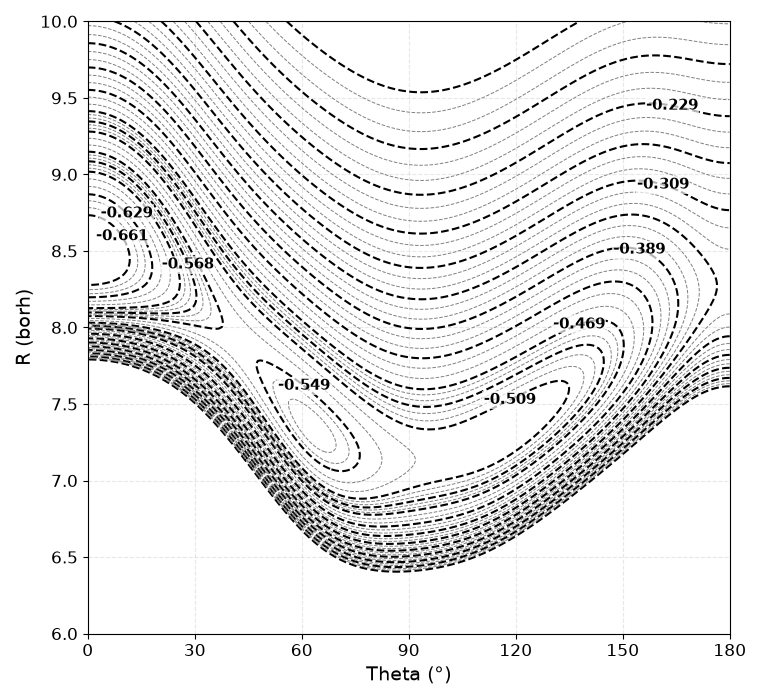
\includegraphics[width=\linewidth]{../Figures/Soutenance/PES-AR-Toczylowski-params.png}
    \end{subfigure}
    \begin{subfigure}{0.49\textwidth}
        \centering
        \caption{Paramètres calculés retenus (\ref{tab:best_params_1})}
        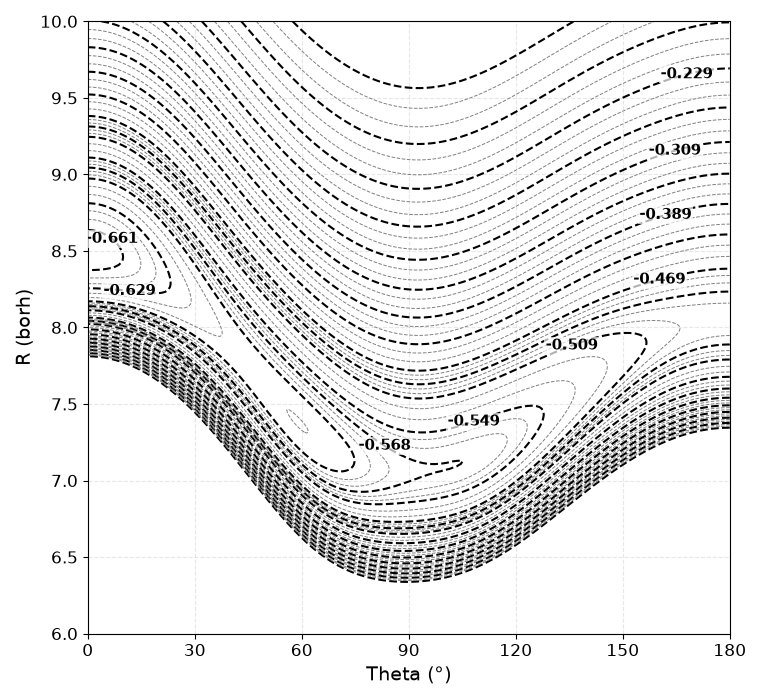
\includegraphics[width=\linewidth]{../Figures/Soutenance/PES-AR-Toczylowski-bestfit.png}
    \end{subfigure}
    \begin{subfigure}{0.55\textwidth}
        \centering
        \caption{Figure de référence \cite{ref1}}
        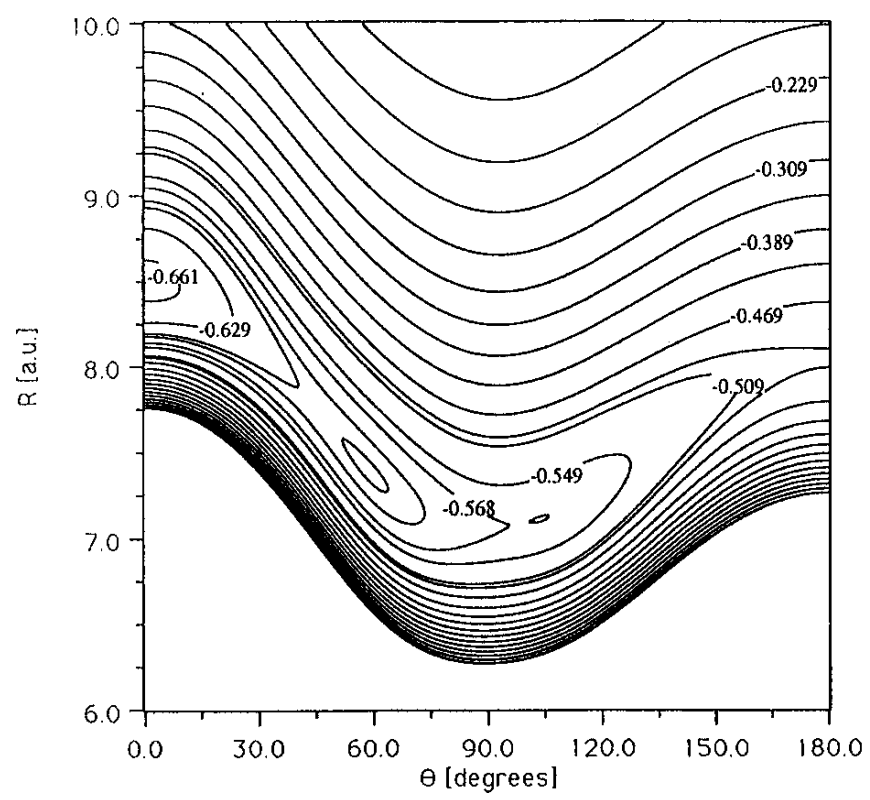
\includegraphics[width=\linewidth]{../Figures/Soutenance/PES-AR-Toczylowski.png}
    \end{subfigure}
\end{figure}

\begin{figure}[H]
  \caption{\centering Coupe de la PES pour $R=7.5\;a_0$ sur quatre configurations de 
  \texttt{least\_squares} avec un même résidu défini par l'erreur absolue -- surface n°2}\label{fig:ls_mauvais_surf2}
  \begin{center}
    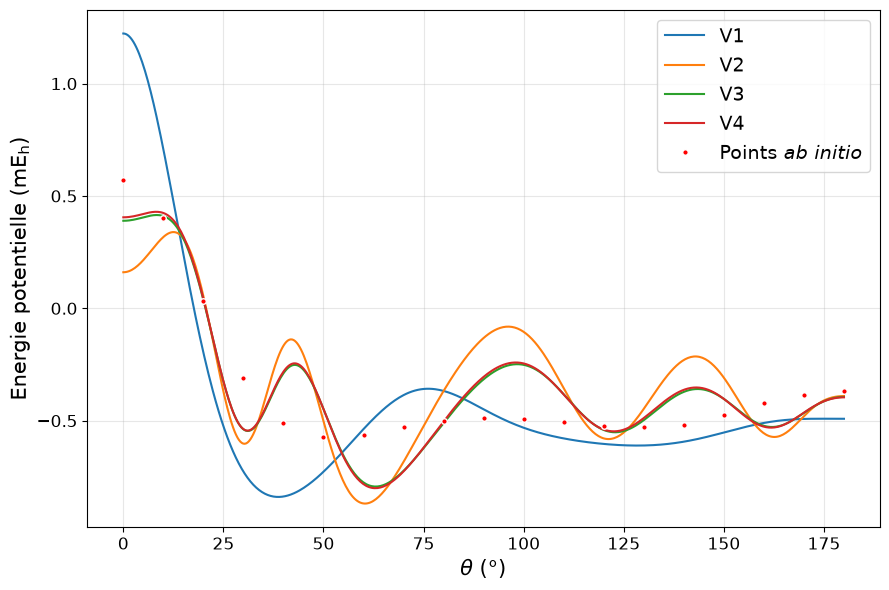
\includegraphics[width=0.95\textwidth]{../Figures/Rapport/surf2-ls1-R7_5.png}
  \end{center}
\end{figure}


\begin{figure}[H]
    \centering
    \caption{\centering Coupes de surface pour $\theta$ fixé -- Ar-HCN (surface n°2)}
    \label{fig:Theta-fixe-surf2}
    \begin{subfigure}{0.65\textwidth}
        \centering
        \caption{$\theta=0$°}
        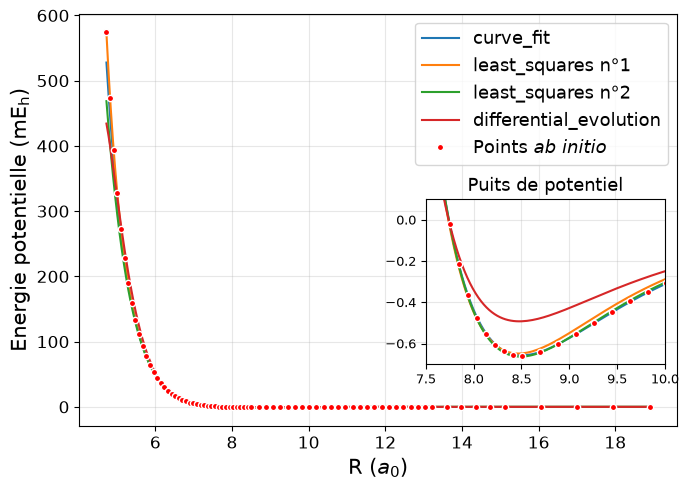
\includegraphics[width=\linewidth]{../Figures/Rapport/surf2-T0.png}
    \end{subfigure}
    \begin{subfigure}{0.65\textwidth}
        \centering
        \caption{$\theta=90$°}
        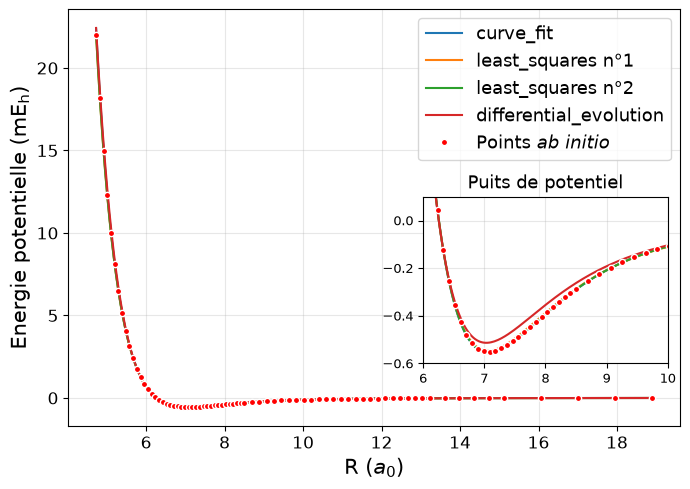
\includegraphics[width=\linewidth]{../Figures/Rapport/surf2-T90.png}
    \end{subfigure}
    \begin{subfigure}{0.65\textwidth}
        \centering
        \caption{$\theta=180$°}
        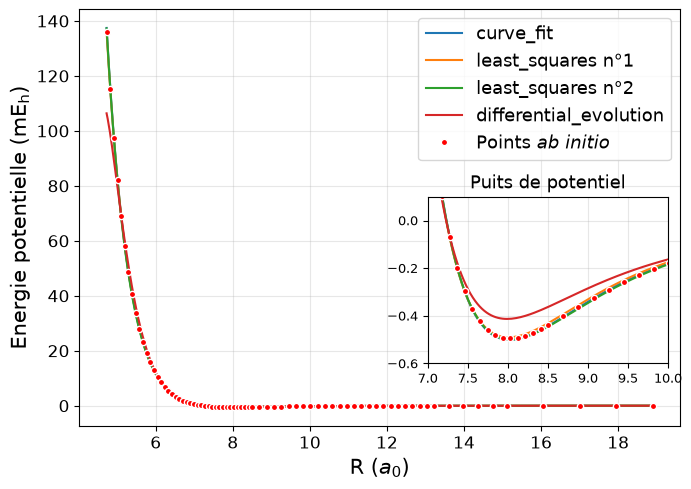
\includegraphics[width=\linewidth]{../Figures/Rapport/surf2-T180.png}
    \end{subfigure}
\end{figure}

\begin{figure}[H]
    \centering
    \caption{\centering Contour plot de l'énergie potentielle pour Ar-HCN (surface n°2)}
    \label{fig:PES-surface-2}
    \begin{subfigure}{0.55\textwidth}
        \centering
        \caption{Paramètres issus de \texttt{least\_squares} n°1}
        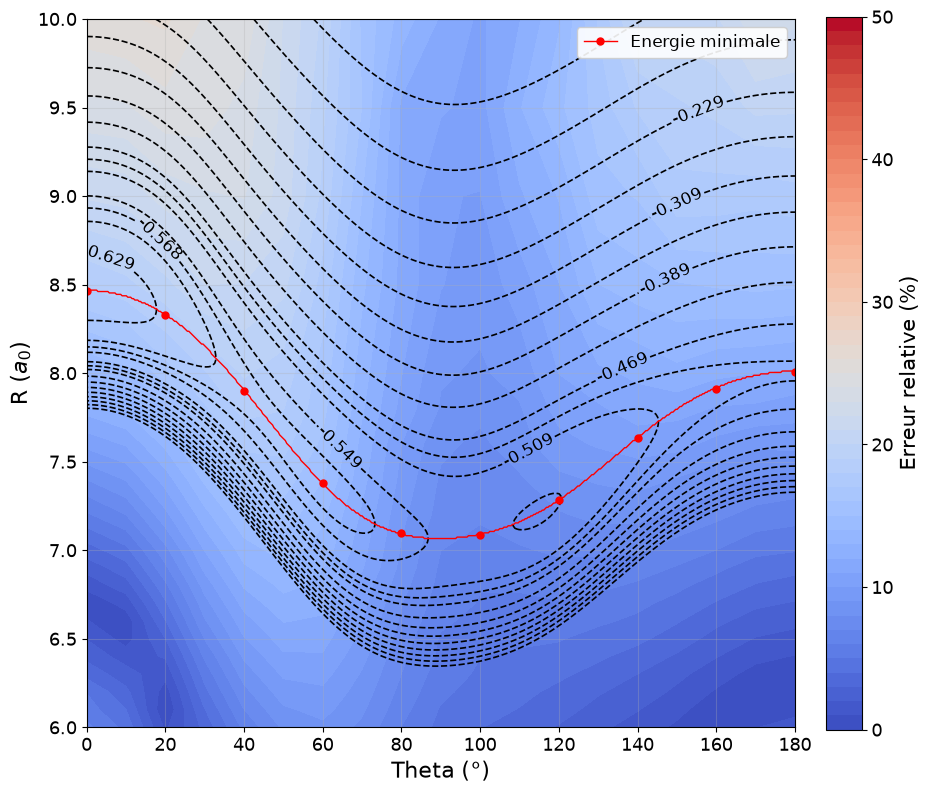
\includegraphics[width=\linewidth]{../Figures/Rapport/PES-surf2-ls1.png}
    \end{subfigure}
    \begin{subfigure}{0.55\textwidth}
        \centering
        \caption{Paramètres issus de \texttt{least\_squares} n°2}
        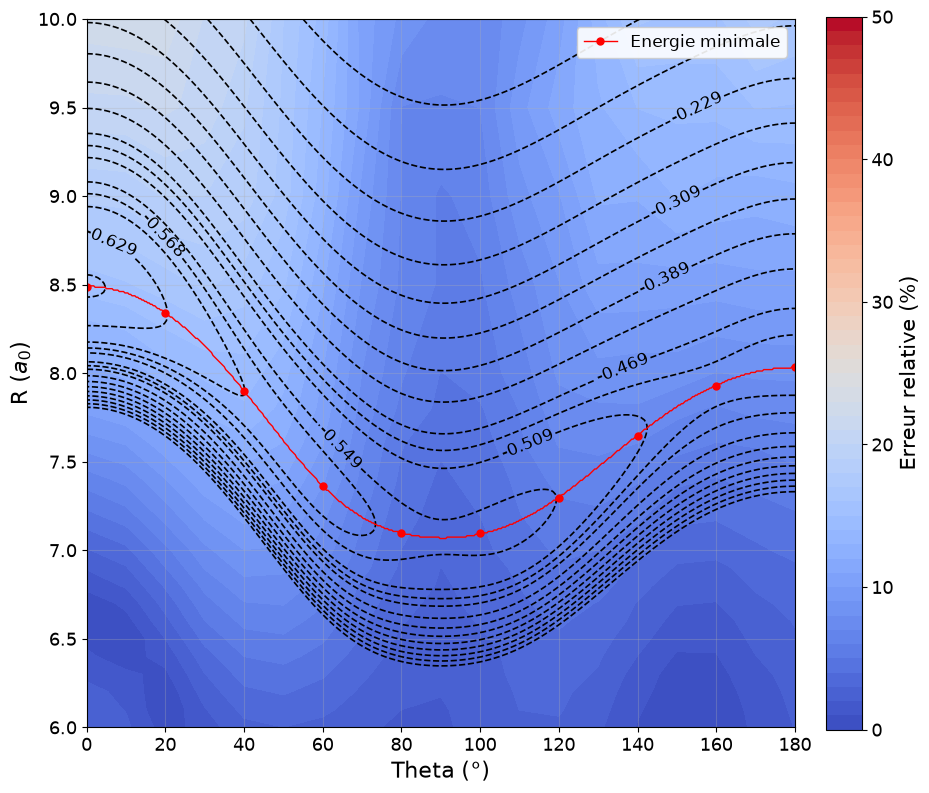
\includegraphics[width=\linewidth]{../Figures/Rapport/PES-surf2-ls2.png}
    \end{subfigure}
    \begin{subfigure}{0.55\textwidth}
        \centering
        \caption{Paramètres issus de \texttt{curve\_fit}}
        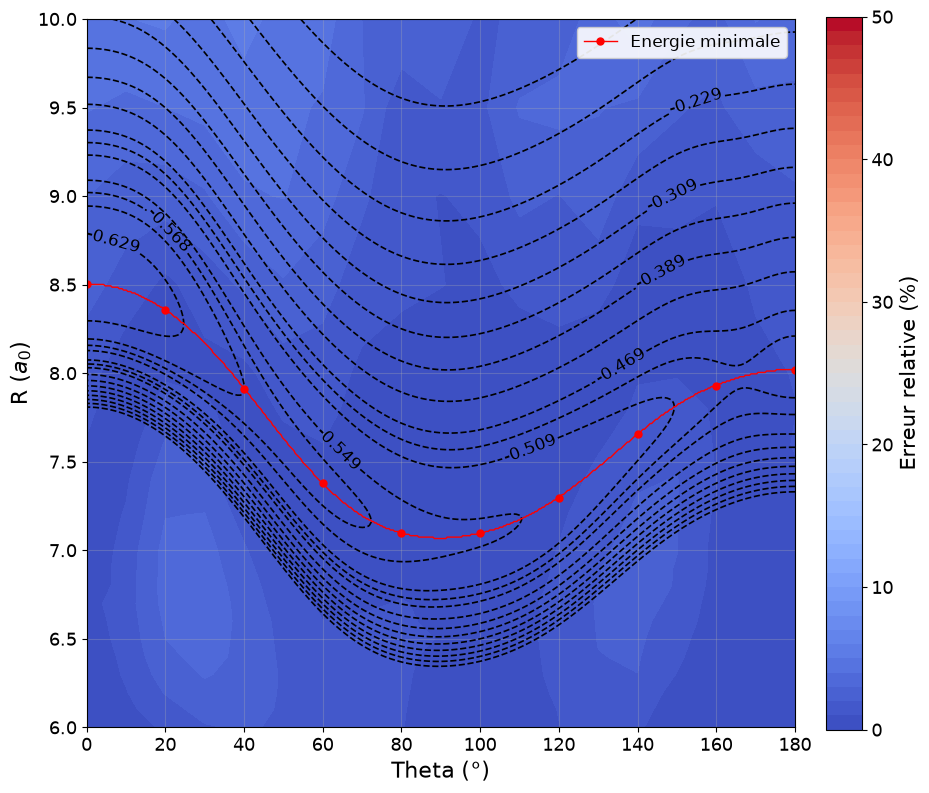
\includegraphics[width=\linewidth]{../Figures/Soutenance/Ar-chinois-contour-err-curve-fit.png}
    \end{subfigure}
\end{figure}

\clearpage{}
\newpage{}
\section{Code Source}

\lstset{
  backgroundcolor=\color{white},     % choose the background color; you must add \usepackage{color} or \usepackage{xcolor}; should come as last argument
  basicstyle=\footnotesize\ttfamily, % the size of the fonts that are used for the code
  breakatwhitespace=false,           % sets if automatic breaks should only happen at whitespace
  breaklines=true,                   % sets automatic line breaking
  captionpos=b,                      % sets the caption-position to bottom
  commentstyle=\color{red},          % comment style
  deletekeywords={...},              % if you want to delete keywords from the given language
  escapeinside={\%*}{*)},            % if you want to add LaTeX within your code
  extendedchars=true,                % lets you use non-ASCII characters; for 8-bits encodings only, does not work with UTF-8
  frame=single,	                     % adds a frame around the code
  framextopmargin=0pt,
  framexbottommargin=0pt,
  keepspaces=true,                   % keeps spaces in text, useful for keeping indentation of code (possibly needs columns=flexible)
  keywordstyle=\bfseries\color{blue},% keyword style
  language=Python,                   % the language of the code
  numbers=left,                      % where to put the line-numbers; possible values are (none, left, right)
  numbersep=5pt,                     % how far the line-numbers are from the code
  numberstyle=\tiny\color{mygray},   % the style that is used for the line-numbers
  rulecolor=\color{black},           % if not set, the frame-color may be changed on line-breaks within not-black text (e.g. comments (green here))
  showspaces=false,                  % show spaces everywhere adding particular underscores; it overrides 'showstringspaces'
  showstringspaces=false,            % underline spaces within strings only
  showtabs=false,                    % show tabs within strings adding particular underscores
  stepnumber=1,                      % the step between two line-numbers. If it's 1, each line will be numbered
  stringstyle=\color{mymauve},       % string literal style
  tabsize=2,	                     % sets default tabsize to 2 spaces
  inputpath=../Fonctions/,                  % subdirectory with C source files
  title=\lstname                     % show the filename of files included with \lstinputlisting; also try caption instead of title
}


\begin{lstlisting}[ caption={Implémentation primaire du modèle analytique de V}, label={lst:V_classique}]
def G(R,Theta,g0,g1,g2,g3):
    g = 0.
    for i in range(6):
        g = g + (g0[i]+g1[i]*R+g2[i]*R*R+g3[i]*R*R*R)
              * eval_legendre(i,math.cos(Theta))
    return g

def X(Theta,x):
    y = 0.
    for i in range(6):
        y = y + x[i] * eval_legendre(i,math.cos(Theta))
    return y

def f(n,x):
    y = 0.
    for k in range(n+1):
        y = y + (x**k)/factorial(k)
    y = 1. - math.exp(-x)*y
    return y

def V(vars, params):

    R, Theta = vars

    Theta_rad = math.radians(Theta)

    b  = params[0:6]    # b0, b1, b2, b3, b4, b5
    c  = params[6:10]   # c0, c1, c2, c3
    d  = params[10:16]  # d0, d1, d2, d3, d4, d5
    g0 = params[16:22]  # g00, g01, g02, g03, g04, g05
    g1 = params[22:28]  # g10, g11, g12, g13, g14, g15
    g2 = params[28:34]  # g20, g21, g22, g23, g24, g25
    g3 = params[34:40]  # g30, g31, g32, g33, g34, g35
        
    abs_BR = math.fabs(X(Theta_rad,b)*R)
    cosTh = math.cos(Theta_rad)
        
    V_sh = G(R,Theta_rad,g0,g1,g2,g3) 
         * math.exp(X(Theta_rad,d)-X(Theta_rad,b)*R)
        
    V_as = f(6,abs_BR) * (c[0]*eval_legendre(0,cosTh)\
                         + c[2]*eval_legendre(2,cosTh))/(R**6)\
         + f(7,abs_BR) * (c[1]*eval_legendre(1,cosTh)\
                         + c[3]*eval_legendre(3,cosTh))/(R**7)
        
    return V_sh + V_as
\end{lstlisting}


\newpage
\begin{lstlisting}[caption={Implémentation optimisée du modèle analytique de V}, label={lst:V_opt}]
import numpy as np
from   numpy.polynomial.legendre import legval
from   scipy.special             import eval_legendre

def f6_opt(x):
    y = 1.0 + x * (1.0 + x * (0.5 + x * (1.0/6.0 + x * (1.0/24.0 + x * (1.0/120.0 + x / 720.0)))))
    return 1.0 - np.exp(-x) * y
def f7_opt(x):
    y = 1.0 + x * (1.0 + x * (0.5 + x * (1.0/6.0 + x * (1.0/24.0 + x * (1.0/120.0 + x * (1.0/720.0 + x / 5040.0))))))
    return 1.0 - np.exp(-x) * y

def V_opt(p, R, Theta):
    R = np.asarray(R, dtype=float)
    cosTh = np.cos(np.deg2rad(np.asarray(Theta, dtype=float)))
    
    b  = p[0:6]
    c  = p[6:10]
    d  = p[10:16]
    g0 = np.asarray(p[16:22], dtype=float)
    g1 = np.asarray(p[22:28], dtype=float)
    g2 = np.asarray(p[28:34], dtype=float)
    g3 = np.asarray(p[34:40], dtype=float)
    
    X_b = legval(cosTh, b)
    X_d = legval(cosTh, d)
    
    X_bR = X_b * R
    abs_BR = np.abs(X_bR)
    
    Pl = eval_legendre(np.arange(6)[:,None],cosTh)

    g = g0[:, None] + R * (g1[:, None] + R * (g2[:, None] + R *  g3[:, None]))  
    
    exp_val = np.clip(X_d-X_bR,-200,200)
    V_sh = np.sum(g * Pl, axis=0) * np.exp(exp_val)

    inv_R = 1.0/R
    inv_R6 = inv_R * inv_R * inv_R * inv_R * inv_R * inv_R
    inv_R7 = inv_R6 * inv_R
    
    V_as = (f6_opt(abs_BR) * legval(cosTh,[c[0],0,c[2]]) * inv_R6
          + f7_opt(abs_BR) * legval(cosTh,[0,c[1],0,c[3]]) * inv_R7)
    
    V_total = V_sh + V_as
    V_total = np.nan_to_num(V_total, nan=1e100, posinf=1e100, neginf=-1e100)
    V_total = np.clip(V_total, -1e100, 1e100)
      
    return V_total
\end{lstlisting}

\newpage
\begin{lstlisting}[caption={Fonction de loss alternative pour le réseau de neurones (Erreur relative)}, label={lst:loss_NN}]
def relative_error_loss(predictions_norm, targets_norm,\
                        E_mean, E_std, epsilon=1.0):
    predictions_raw = (predictions_norm * E_std) + E_mean
    targets_raw = (targets_norm * E_std) + E_mean

    erreur_absolue = torch.abs(predictions_raw - targets_raw)
    
    erreur_relative = erreur_absolue / (torch.abs(targets_raw) + epsilon)
    
    return torch.mean(erreur_relative)
\end{lstlisting}
\end{document}
